\documentclass{report}

\usepackage{amsmath, amsthm, amssymb, amsfonts}
\usepackage{thmtools}
\usepackage{graphicx}
\usepackage{setspace}
\usepackage{geometry}
\usepackage{float}
\usepackage{hyperref}
\usepackage[utf8]{inputenc}
\usepackage[english]{babel}
\usepackage{framed}
\usepackage[dvipsnames]{xcolor}
\usepackage{tcolorbox}
\usepackage{multicol}
\usepackage{subfig}
\usepackage{wrapfig}

\colorlet{LightGray}{White!90!Periwinkle}
\colorlet{LightOrange}{Orange!15}
\colorlet{LightGreen}{Green!15}

\newcommand{\HRule}[1]{\rule{\linewidth}{#1}}

\declaretheoremstyle[name=Theorem,]{thmsty}
\declaretheorem[style=thmsty,numberwithin=section]{theorem}
\tcolorboxenvironment{theorem}{colback=LightGray}

\declaretheoremstyle[name=Proposition,]{prosty}
\declaretheorem[style=prosty,numberlike=theorem]{proposition}
\tcolorboxenvironment{proposition}{colback=LightOrange}

\declaretheoremstyle[name=Principle,]{prcpsty}
\declaretheorem[style=prcpsty,numberlike=theorem]{principle}
\tcolorboxenvironment{principle}{colback=LightGreen}

\setstretch{1.2}
\geometry{
    textheight=9in,
    textwidth=5.5in,
    top=1in,
    headheight=12pt,
    headsep=25pt,
    footskip=30pt
}

% ------------------------------------------------------------------------------
\tcbset{
    sharp corners,
    colback = white,
    before skip = 0.2cm,    % add extra space before the box
    after skip = 0.5cm      % add extra space after the box
}                           % setting global options for tcolorbox

\definecolor{main}{HTML}{5989cf}    % setting main color to be used
\definecolor{sub}{HTML}{cde4ff}     % setting sub color to be used

\newtcolorbox{boxH}{
    colback = sub, 
    colframe = main, 
    boxrule = 0pt, 
    leftrule = 6pt % left rule weight
}

\newcommand{\SubItem}[1]{
    {\setlength\itemindent{15pt} \item[-] #1}
}

% ------------------------------------------------------------------------------

\begin{document}

% ------------------------------------------------------------------------------
% Cover Page and ToC
% ------------------------------------------------------------------------------

\title{ \normalsize \textsc{}
		\\ [2.0cm]
		\HRule{1.5pt} \\
		\LARGE \textbf{\uppercase{Hardware and Device-to-Device Communication Security}}
		\HRule{2.0pt} \\ [0.6cm] \LARGE{Notes about that} \vspace*{10\baselineskip}}
\date{}
\author{\textbf{Fabio Lorenzato}} 
		

\maketitle
\newpage

\tableofcontents
\newpage

% ------------------------------------------------------------------------------

% \section{Examples}

% \begin{theorem}
%     This is a theorem.
% \end{theorem}

% \begin{proposition}
%     This is a proposition.
% \end{proposition}

% \begin{principle}
%     This is a principle.
% \end{principle}

% Maybe I need to add one more part: Examples.
% Set style and colour later.

% \newpage
\part{Wireless}
\chapter{Digital Communication}
This first section is all about how to convert and transmit some signal.
\begin{section}{Introduction}
\label{sec:intro}
The goal of communication is to transmit some kind of data form a sender to a receiver. In order 
to do so, the physical layer defines the means of transmitting a stream of \textbf{raw bits} over a
physical data link, which connects those two nodes.\\
Data is transmitted in the form of \textbf{signals}, which are a physical representation of the data.
The signal is transmitted over a \textbf{channel}, which is the transmission medium that connects 
the sender and receiver. This can be both wired or wireless.\\
% Whereas with wired channels, checking the device connected to the channel is easier to implement, 
% with wireless ones security is a major when travelling in the channel. This is for may reasons:
In wired channels, it is really easy to check which devices are connected to the channel, on the
other hand, in wireless channels the communication is broadcast, and security becomes a major
concern. This is for many reasons:
\begin{itemize}
  \item No inherent protection is applied to the channel( it is replaced by a logical association)
     \subitem sending and receiving messages do not need physical access to the network 
     infrastructure
  \item the communication is in broadcast, which is intrinsic of radio nature.
    \subitem Transmission can be overheard by anyone in range( which can be quite big, depending 
    on the situation), and anyone can generate a transmission, for example by jamming nearby 
    transmissions.
\end{itemize}
As a result:
\begin{itemize}
  \item Eavesdropping is easy
  \item Injecting fake messages into the communication in easy
  \item replaying previously recorded messages is easy(\textit{meaconing}). This is actually very 
    dangerous for gps positioning, so it is also a security concern.
  \item illegitimate access to the network and its services is easy
  \item Denial of service attacks are easy, achieved by jamming the channel.
\end{itemize}
% 9/43
\end{section}
\begin{section}{Digital Communication System}
The digital communication system in characterized by three sections: 

\begin{itemize}
  \item the \textbf{user section}, which consist in the transmitter and the receiver, that want to 
    communicate. 
  \item the \textbf{interface section}, which is the interface to conveying the signal from the 
    user to the analog channel. It also transforms bits to analog signal, compressing and encoding 
    them, also associating bits to signal waveforms, to transform bits to analog signal.
  \item the \textbf{channel section}, which is the physical medium, that can only propagate analog 
    waveforms. In the end, we want to transmit digital signal but we are forced to use analog ones.
\end{itemize}

\begin{figure}[h]
  \centering
  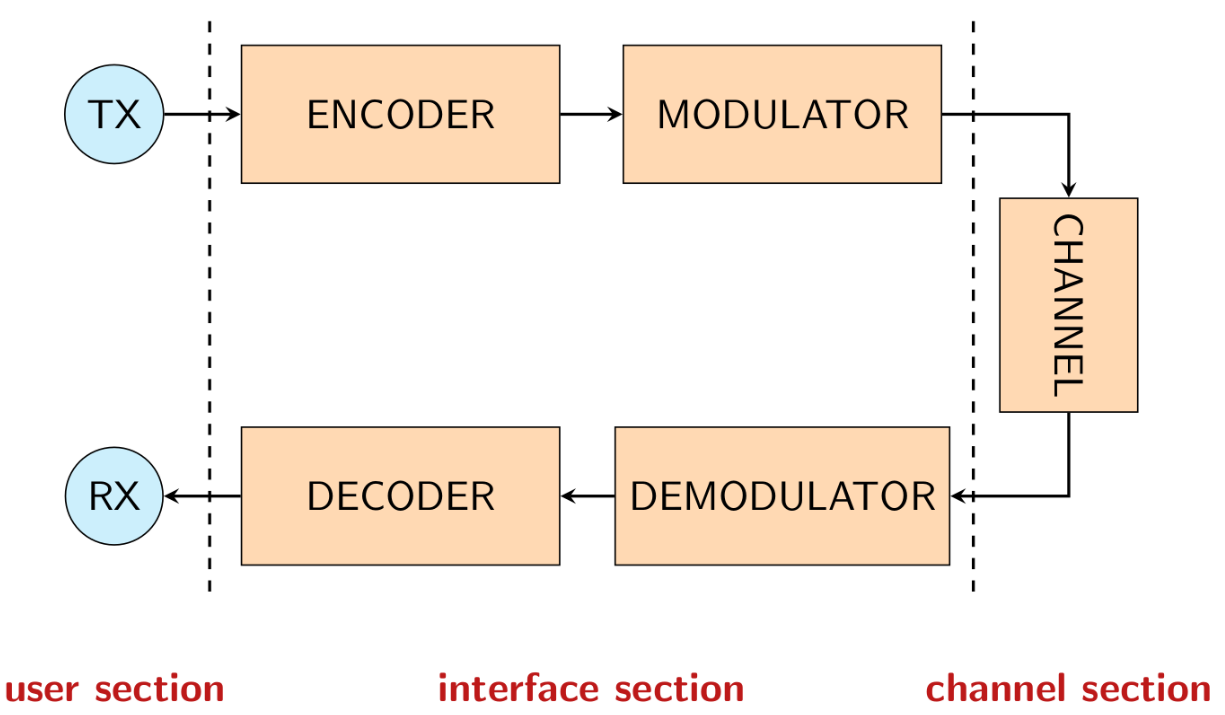
\includegraphics[width=0.7\textwidth]{img/wireless/digital communication schema.png}
  \caption{Digital Communication System}
  \label{fig:Digital Communication System}
\end{figure}
\begin{subsection}{The transmitter chain}
The transmitter chain is the part of the system that takes the digital signal, or an analog one 
converted to digital, and converts it to an analog signal, that can be transmitted over the
channel.\\
It is basically composed by two parts. The first one being an \textbf{encoder}, which can limit the amount 
of bits transmitted(\textit{source encoding}), and/or make the transmitted sequence more robust to
errors(\textit{channel encoding}).\\
The second one is the \textbf{modulator}, which is the part of the system that takes the digital
signal and converts it to an analog one to transmit it over the channel.
\end{subsection}

\begin{subsection}{The channel}
  \label{subsec:channel}
The channel is the physical medium that transfers bits from interface to interface, from the sender
to the receiver.
Its operation is affected by different types of disturbances such as:
\begin{itemize}
	\item frequency-domain distortion
	\item wireless fading
	\item additive noise
	\item impulsive noise
	\item interference from other frequency channels (interchannel interference)
	\item interference from the same frequency channel (cochannel interference)
	\item Intentional interference
\end {itemize}
\end{subsection}
\begin{subsection}{The receiver chain}
The receiver chain is the part of the system that takes the analog signal from the channel and
converts it to a digital signal, that can be processed by the user.\\
It is composed by the dual counterpart of the transmitter chain, the \textbf{demodulator} and the
\textbf{decoder}. \\
The demodulator takes the analog signal and converts it to a sequence of samples that can be
processed by the decoder.\\
The decoder takes the sequence of samples and converts it to a digital signal. It implements
\textit{channel decoding}, to correct errors, and \textit{source decoding}, to recover the original
message.
\end{subsection}
\end{section}

\begin{section}{Signal representation and Processing}
  \begin{boxH}
    A \textbf{signal} is a (mathematical) function that conveys information about a phenomenon.
  \end{boxH}
  Basically, any quantity that varies over space or time can be used to represent a informations,
  allowing to describe the evolution of physical quantities over time(voltages, currents, \dots).\\
  Its mathematical representation is therefore a function of real variable (time) taking real or 
  complex(more than one) values.\\
  We will be mostly focused on Electromagnetic Signals (e.g. voltage), but the general concepts 
  can be applied to any kind of signal
  \begin{subsection}{Energy of a signal}
    The energy of a signal is the integral of the squared modulus of the signal itself.
    \begin{equation}
      E(x) = \int_{-\infty}^{\infty} |x(t)|^2 dt
    \end{equation}
    As we can see , the energy is a scalar value, and the whole function is made positive by the
    squared modulus.\\
    \begin{figure}[h]
      \centering
      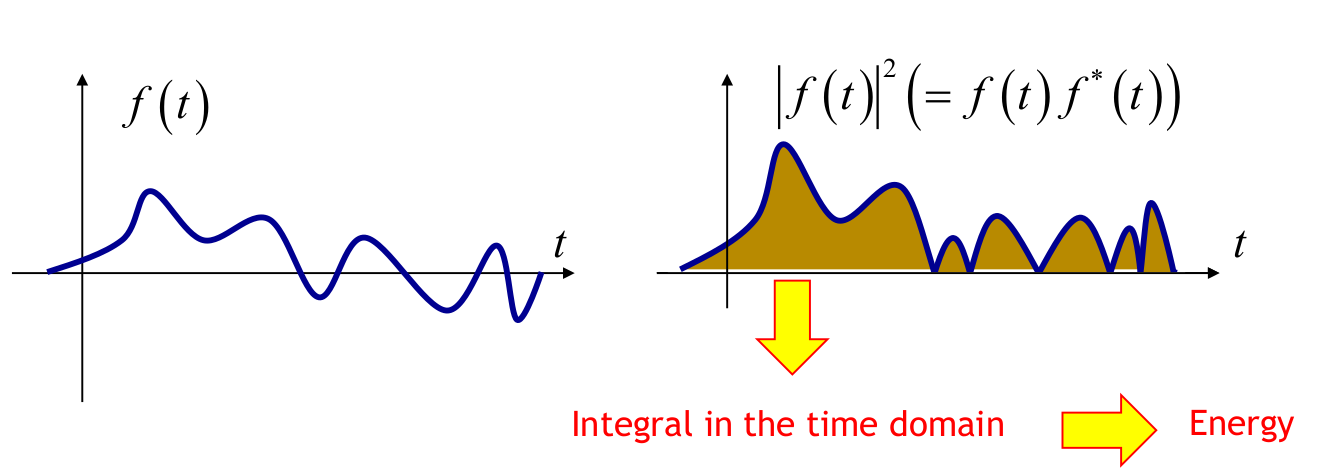
\includegraphics[width=0.7\textwidth]{img/wireless/energy signal.png}
      \caption{Energy of a signal}
      \label{fig:Energy of a signal}
    \end{figure}
    A signal with a very large amplitude, over time, will have a very high energy, while a signal
    which assumes values close to zero will have a very low energy, being a very weak signal.\\
    Furthermore, we can notice that the higher the distance of the signal from the origin, the
    larger the energy.
  \end{subsection}
  \begin{subsection}{Power of a signal}
    When we refer to power we can refer to the \textbf{instantaneous power} of a signal, which is just the 
    square module of a signal
    \begin{equation}
      P(x) = |x(t)|^2
    \end{equation}
    but much more commonly we refer to the average power of a signal, which is the time average of
    the instantaneous power of the whole signal.
    \begin{equation}
      P(x) = \lim_{a \to \infty} \frac{1}{2a} \int_{-a}^{a} |x(t)|^2 dt
    \end{equation}
    This a again a scalar value.
  \end{subsection}
  \begin{subsection}{Signal Representation}
    To analyze and process the signals, it is necessary to adequately represent them, and the
    definition of signals as "time functions" is NOT effective for many applications, for many 
    reasons.\\
    Generally, signals can become very complicated depending on our communication system, and
    we want different ways of representing them, to make them easier to process.\\
    For instance, we can represent a signal as a sum of elementary signals, thanks to the scalar
    product of the signal with a basis of the space of signals.\\

    The scalar product between signals is a scalar value, which is a measure of the similarity 
    among signals.\\
    If two function are quite similar we will get a large number.
    It it is zero, they are said to be orthogonal.
    \begin{equation}
      \langle x,y \rangle = \langle x(t),y(t) \rangle = \int_{-\infty}^{\infty} x(t)y^*(t) dt
    \end{equation}

    So, if we have a set of elementary signals $w_1(t), w_2(t), \dots, w_m(t)$, we write the signal
    $x(t)$ as a linear combination of the elementary signals:
    \begin{equation}
      x(t) = \sum_{i=1}^{m} \alpha_i w_i(t)
    \end{equation}
    where $\alpha_i$ are the coefficients of the linear combination $\alpha_i = \langle x(t), 
    w_i(t) \rangle$.\\
    In a more down to hearth way, the coefficient $\alpha_i$ allows us to understand how much each
    individual signal is similar to any other elementary signal we are considering, and because the 
    scalar product is higher for similar signals, we can understand how much each elementary signal
    is contributing to the whole signal.\\

    Furthermore, by adjusting the coefficient, we are able to create a whole different signal using
    the same elementary signals.
    \begin{subsubsection}{A common example: In Phase and Quadrature components representation}
      \label{sub:IQ representation}
      Lets consider a very simple basis, or a set of elementary signals, which is actually more 
      important that many other ones:
      \begin{itemize}
        \item the \textbf{in-phase} signal, which, in this case, is a cosine function $w_1(t) = cos(2\pi f_o t)$
        \item the \textbf{quadrature} signal, which, in this case, is a sine function $w_2(t) = sin(2\pi f_o t)$
      \end{itemize}
      where $f_o$ is the frequency, in Hz, of the signal.\\
      We can write any signal as a linear combination of these two signals, just by adjusting the
      coefficients:
      \begin{equation}
        x(t) = x_1 cos(2\pi f_o t) + x_2 sin(2\pi f_o t)
      \end{equation}
      where x(t) is the signal we want to represent, and $x_1$ and $x_2$ are the coefficients of the
      linear combination.\\

      A very simple representation of this complex signal is obtainable by representing each signal 
      as an axes in a complex plane, for example in figure \ref{fig:Complex Plane} the x-axis 
      is the in-phase signal, and the y-axis is the quadrature signal.\\
      Each signal can be represented as a point in the complex plane, because the distance from the
      origin signal(\textit{axis}) is the amplitude of the signal.\\
      This kind of representation is called the \textbf{In-phase and Quadrature} representation, or
      \textbf{I/Q} representation.\\
      For example, choosing a point close to the x-axis, we are choosing a signal with a very low
      quadrature component, and a very high in-phase component.Furthermore, a set of those 
      different points is called a \textit{constellation}\\
      \begin{figure}[h]
        \centering
        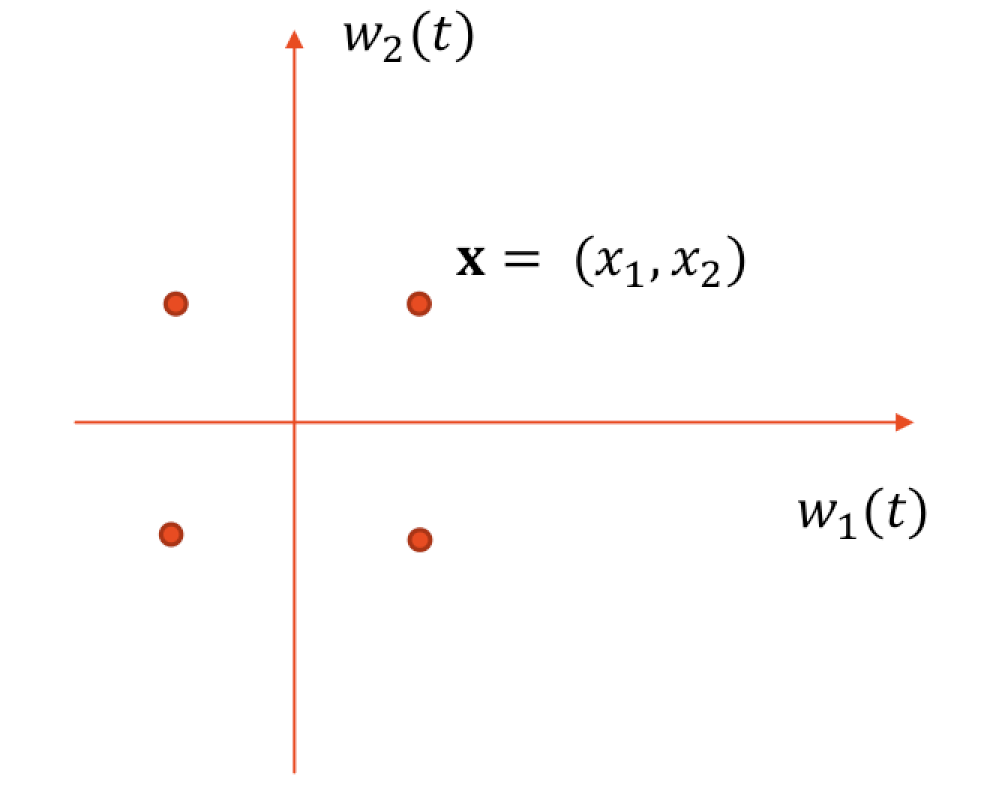
\includegraphics[width=0.5\textwidth]{img/wireless/iq representation.png}
        \caption{Some points that represent some signals in the I/Q representation}
        \label{fig:Complex Plane}
      \end{figure}
    \end{subsubsection}
  \end{subsection}
  \begin{subsection}{Fourier Analysis}
    Lets consider a signal with base the complex exponential functions 
    \begin{equation}
      e^{j2\pi \frac{n}{T} t} = cos(2\pi \frac{n}{T} t) + j sin(2\pi \frac{n}{T} t)
      \label{euler formula}
    \end{equation}
    It is actually characterized by a frequency $f_n = \frac{n}{T}$, where T is the period of the
    signal. The higher the frequency, the more oscillations we will have in the same time interval.
    In this function they have both the same frequency.\\

    We can use that function as a basis to decompose a signal, again. This is because it is 
    possible to generate an infinite set of functions
    \begin{equation}
      w_n(t) = \frac{1}{\sqrt{T}} e^{j\frac{2\pi}{T} nt} 
    \end{equation}
    with $-T/2 \leq t \leq T/2$, each associated with a frequency.
    That can be used ad a complete basis for all the signals limited in $[-T/2, T/2]$ or periodic.\\
    For example, we can write a signal as a linear combination of these functions:
    \begin{equation}
      x(t) = \frac{1}{\sqrt{T}} \sum_{n=-\infty}^{\infty} c_n e^{j\frac{2\pi}{T} nt}
      \label{Fourier Series}
    \end{equation}
    where $c_n$ are the coefficients of the linear combination $c_n = \langle x(t), w_n(t) \rangle$.\\
    Each one of those coefficients is a measure of how much each frequency $f_n$, of the $n$-th
    sinusoid(the shape of equation \ref{euler formula}) is present in the signal $x(t)$.\\
    \begin{figure}[h]
      \centering
      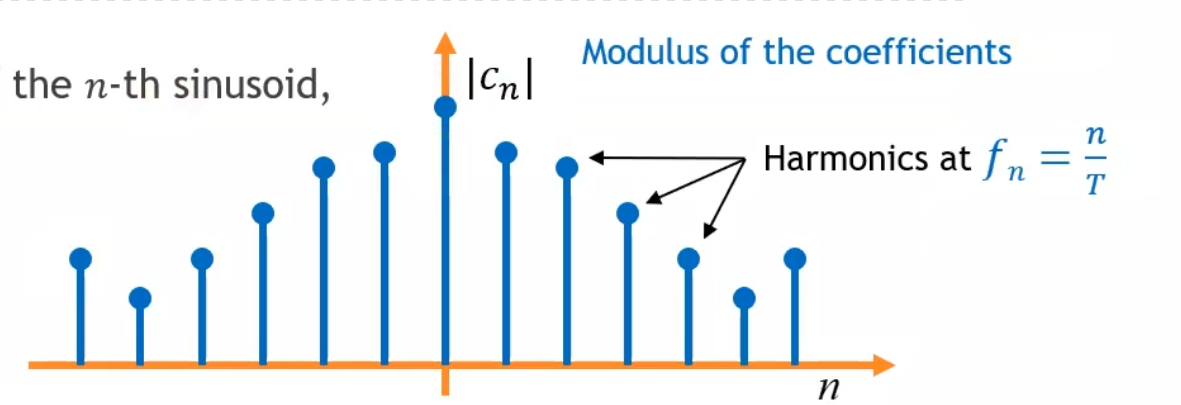
\includegraphics[width=0.7\textwidth]{img/wireless/euler plot.png}
      \caption{Plot of the coefficients of equation \ref{Fourier Series}}
      \label{fig:Fourier Analysis}
    \end{figure}
    Lets now take a look at picture \ref{fig:Fourier Analysis}. We can see that the coefficients
    are higher when the frequence is very small, so the signal \ref{Fourier Series} is mostly
    composed by large components of low frequency.\\
    This whole concept is called \textbf{Fourier Analysis}, or frequency analysis, which allows
    to decompose a signal into a set of frequencies.
    \begin{boxH}
    TLDR: I can build a signal trough a combination of frequency components. \\
    The coefficients of this frequency components are the measure of how much each frequency is 
    present in the signal.
    \end{boxH}
    Now we just need to expand it to any signal and any frequency( a continuous frequency domain).
    By doing so we can derive the definition of the \textbf{Fourier Transform} of a signal $x(t)$:
    \begin{equation}
      X(f) = \int_{-\infty}^{\infty} x(t) e^{-j2\pi ft} dt
      \label{Fourier Transform}
    \end{equation}
    where $X(f)$ is the Fourier Transform of the signal $x(t)$, and $f$ is the frequency.\\
    The Fourier transform is equivalent to a scalar product between the signal and the complex
    exponential function at a given frequency $f$. This means that each of the values of the
    Fourier Transform is a measure of how much the frequency $f$ is present in the signal $x(t)$.\\
    Furthermore, trough the inverse of equation \ref{Fourier Transform}
    \begin{equation}
      x(t) = \int_{-\infty}^{\infty} X(f) e^{j2\pi ft} df
      \label{Inverse Fourier Transform}
    \end{equation}
    we can write again a signal $x(t)$ as a linear combination of the complex exponential functions
    , which represents the frequency components of the signal, weighted by the Fourier Transform.\\
      
    \begin{boxH}
      The Fourier Transform $X(F)$ indicates the "weight" of each frequency component( sinusoidal
      component at a given frequency $f$) in the signal $x(t)$.\\
      The inverse Fourier Transform $x(t)$ tells us we can decompose any signal into frequency 
      components( sinusoidal components at a given frequency $f$).
    \end{boxH}
    
    \begin{figure}[h]
      \centering
      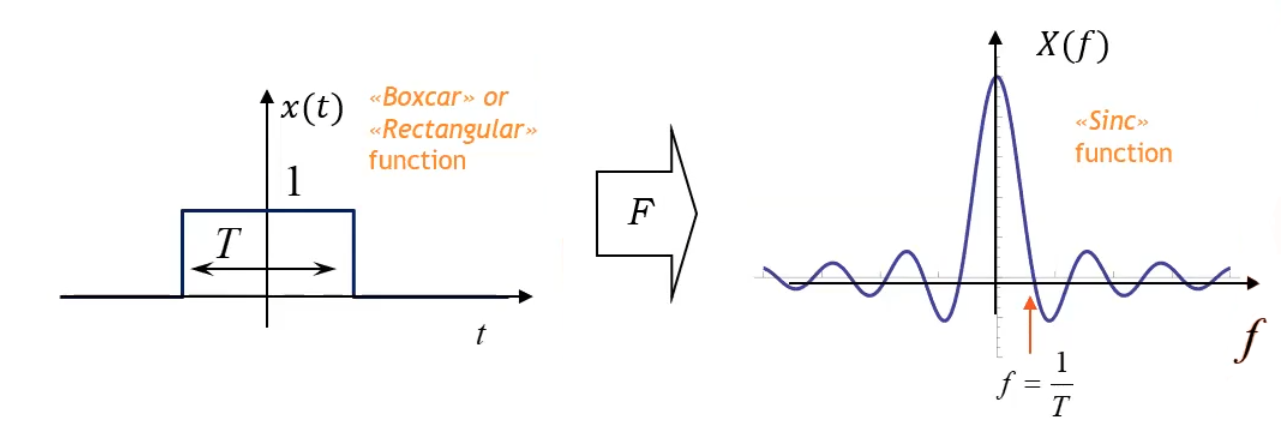
\includegraphics[width=0.9\textwidth]{img/wireless/fourier square function.png}
      \caption{Fourier Transform of a square function}
      \label{fig:Fourier Transform}
    \end{figure}

    With that in mind, take a look at figure \ref{fig:Fourier Transform}. It represents a rectangular
    signal (a signal that is 1 for a certain time, and 0 for the rest of the time), and its Fourier
    Transform, which tells us the frequency components of the signal.\\
    From that, we can see that the Fourier Transform is mostly composed by low frequency components,
    because values closer to zero are higher. That is because in the constant part of the signal
    has a sinusoidal component that constant.

    \begin{boxH}
      To wrap it up, for each signal we have a \textbf{spectral representation}. And for each operation
      over a signal, there are equivalents effects in the frequency domain.\\
      Furthermore, a signal that has finite duration in time, has a infinite support in the frequency
      domain.
    \end{boxH}
  \end{subsection}
  \begin{subsection}{Bandwidth}
    The bandwidth is the \textbf{interval of frequencies} that a signal occupies.\\
    If we consider a signal $x(t)$, we can define the bandwidth as the interval of frequencies
    where the Fourier Transform $X(f)$ is different from zero. \\ 
    Signals have often infinite support over the frequency domain over a finite duration, but many 
    of them are characterized by a quasi-null(finite) spectrum outside a certain interval of 
    frequencies( the main lobes of the spectrum).\\
    For this reason, we usually consider the bandwidth around half of the frequency spectrum of the
    signal, as shown in figure \ref{fig:Bandwidth}(for example 3dB bandwidth, or half power 
    bandwidth).\\
    \begin{figure}[h]
      \centering
      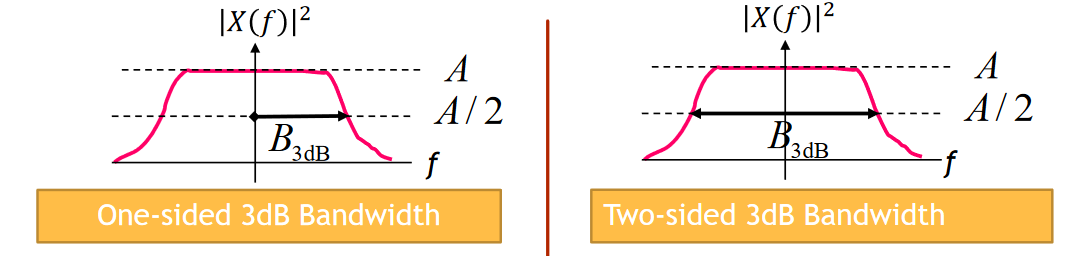
\includegraphics[width=0.8\textwidth]{img/wireless/bandwidth.png}
      \caption{Bandwidth of a signal}
      \label{fig:Bandwidth}
    \end{figure}
    \begin{subsubsection}{Bandwidth in linear systems}
      A \textbf{system} is a set of operations applied to signals.\\
      The relationship between the bandwidth of the input signal and the bandwidth of a system is
      usually very important. In fact, when a system is used to pass or remove particular 
      frequencies of a signal, it can be regarded as a system.\\
      We can associate a bandwidth to a system, specifically a \textbf{linear-time invariant} system,
      with a \textbf{frequency response} $H(f)$.This mean that we can associate a bandwidth to a
      system, making us able to compute a new bandwidth $Y(f)$ by combining together the bandwidth 
      $X(f)$ of the input signal and the frequency response $H(f)$ of the system($Y(f) = X(f)H(f)$
      in formulas).\\
      This concept can be represented graphically very easily, like in figure 
      \ref{fig:Bandwidth System}. If the result of the combination of the input signal and the
      sequence of operation of the system is a signal with a bandwidth $Y(f)$. If the bandwidth of 
      the linear system is larger than the origin signal, the signal pass trough smoothly($Y(f) \approx X(f)$).\\
      However, if the bandwidth of the signal is larger than the bandwidth of the system, the signal
      will be cutted off($Y(f) \ne H(f)$).\\

      \begin{figure}[h]
        \centering
        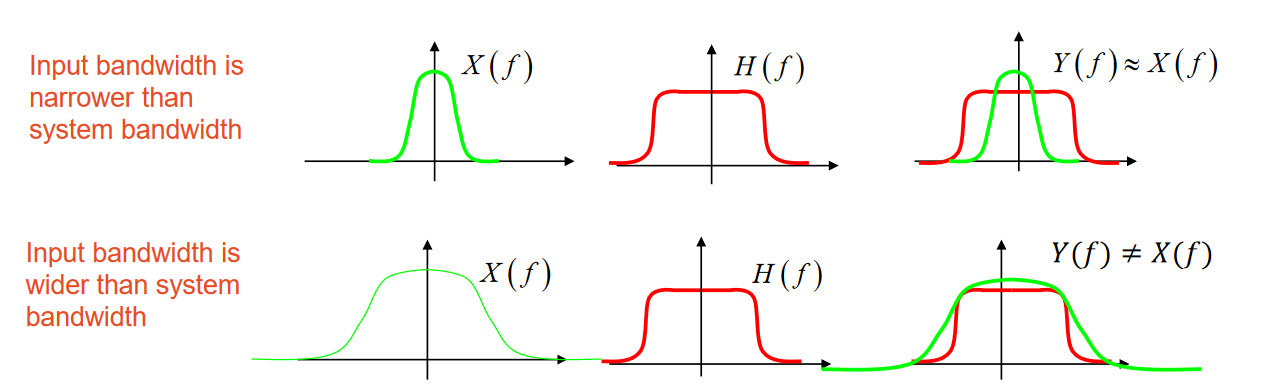
\includegraphics[width=0.8\textwidth]{img/wireless/bandwidth system.png}
        \caption{Bandwidth of a system}
        \label{fig:Bandwidth System}
      \end{figure}
    \end{subsubsection}
  \end{subsection}

  \begin{subsection}{Filters}
    A filter is a system used to model desired and undesired effects over a signal.\\
    It is usually used to remove undesired frequency components from a signal, but overall can be
    used to:
    \begin{itemize}
      \item share the wireless medium
      \item model the spectrum of a signal over the channel
      \item mitigate undesired effects over a signal trough equalizers
    \end{itemize}
    \end{subsection}
    \begin{subsection}{Signal modulation}
      Signal modulation is the process of multiplying a signal by a sinusoidal function, resulting
      in a \textbf{frequency shift}.
      \begin{equation}
        y(t) = x(t) \cdot cos(2\pi f_0 t)
      \end{equation}
      This is possible because
      \begin{equation}
        F(x(t) \cdot cos(2\pi f_0 t)) = \frac{1}{2}[X(f-f_0) + X(f+f_0)]
      \end{equation}
      where $X$ is the frequency domain representation.\\ 
      \begin{figure}[h]
        \centering
        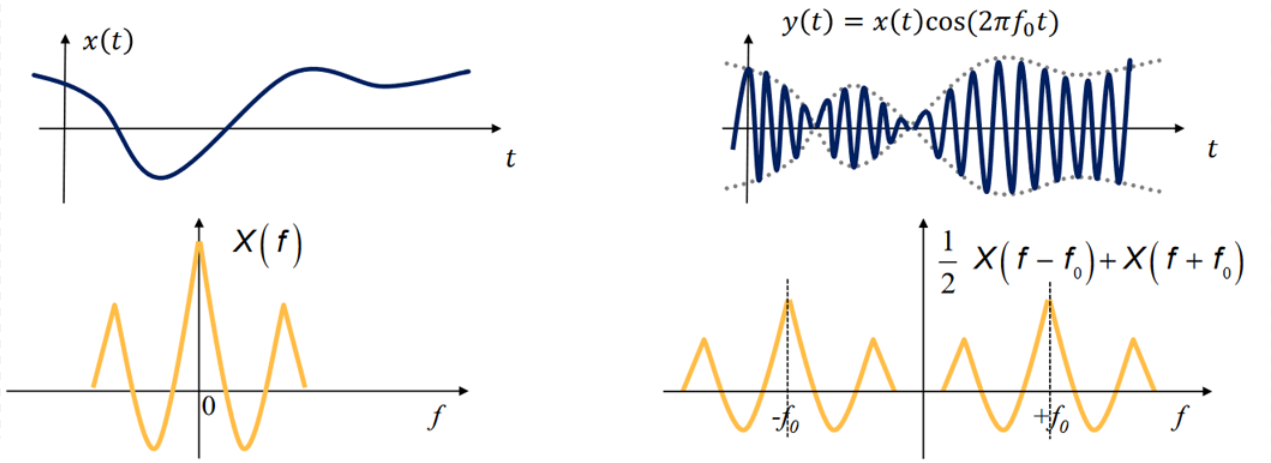
\includegraphics[width=0.8\textwidth]{img/wireless/signal modulation.png}
        \caption{Graphical representation of the modulation}
        \label{fig:Modulation}
      \end{figure}
      We can see that as a result of the modulation, the spectrum of the signal is shifted around
      the frequency $f_0$, as shown in figure \ref{fig:Modulation}.\\

    \end{subsection}
    \begin{subsection}{Signal demodulation}
      When modulating a signal, we alter it a bit, centering it around the frequency $f_0$, shifting
      the spectrum of the signal. The effect of this operation is not trivial.\\
      To recover the original signal, we need to multiply the modulated signal by a sinusoidal
      function at the same frequency $f_0$ as the one used for the modulation. This allows us to
      shift the spectrum back to the original position.\\
      This operation is called \textbf{demodulation}.\\
      A given modulated signal $Y(f)$
      \begin{equation}
        Y(f) = \frac{A}{2}[X(f-f_0) + X(f+f_0)]
      \end{equation}
      shown in figure \ref{fig:Demodulation1}
      \begin{figure}[h]
        \centering
        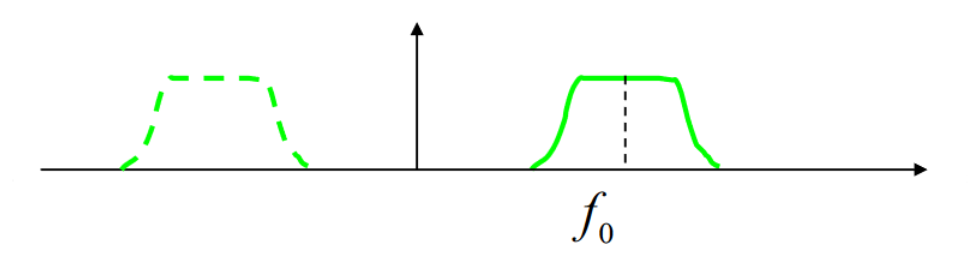
\includegraphics[width=0.8\textwidth]{img/wireless/demodulation1.png}
        \caption{A modulated signal at frequency $f_0$}
        \label{fig:Demodulation1}
      \end{figure}
      can be demodulated by multiplying it by the same sinusoidal function used for the modulation
      \begin{equation}
        Y'(f) = Y(f) \cdot cos(2\pi f_0 t)= \frac{A}{2}X(f)+\frac{A}{4}[X(f-2f_0)+X(f+2f_0)]
      \end{equation}
      shown in figure \ref{fig:Demodulation2}\\
      \begin{figure}[h]
        \centering
        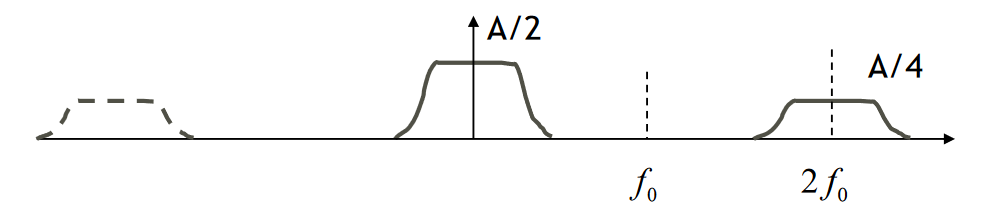
\includegraphics[width=0.8\textwidth]{img/wireless/demodulation2.png}
        \caption{A demodulated signal at frequency $f_0$}
        \label{fig:Demodulation2}
      \end{figure}
      This doesn't allow us to recover the original spectrum of the signal.
      That's why we need to use a \textbf{low-pass filter} to remove the frequency components at
      $2f_0$ and its symmetrical counterpart, as shown in figure \ref{fig:Demodulation3}.\\
      \begin{figure}[h]
        \centering
        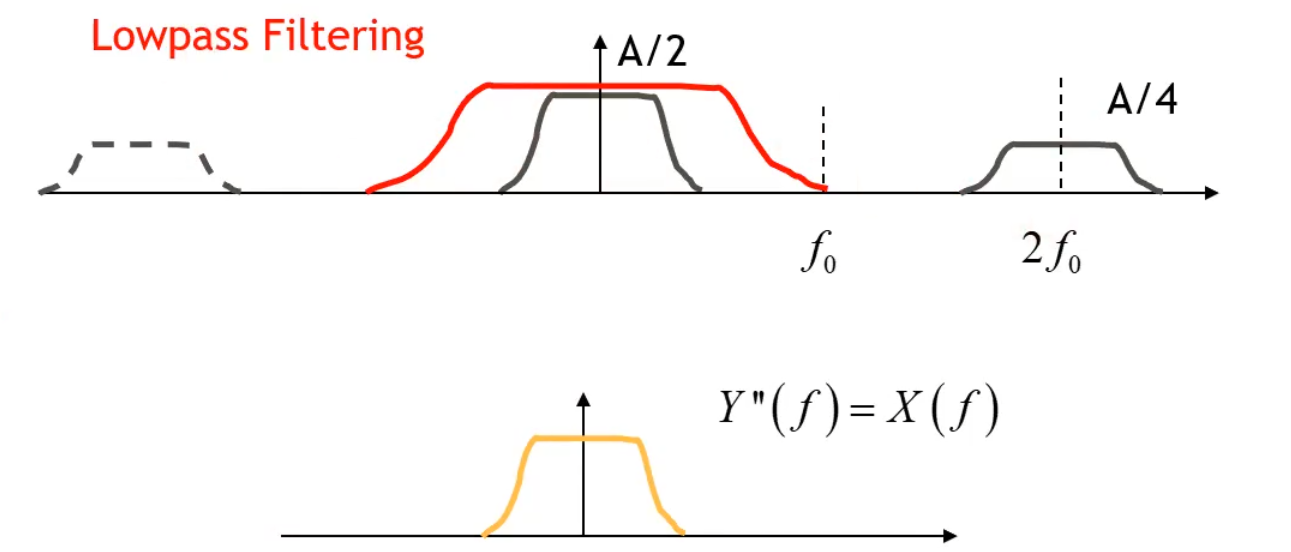
\includegraphics[width=0.8\textwidth]{img/wireless/demodulation3.png}
        \caption{A demodulated signal at frequency $f_0$ after a low-pass filter}
        \label{fig:Demodulation3}
      \end{figure}

    \end{subsection}
    \begin{subsection}{Frequency Multiplexing(FDM)}
      \label{subsec:FDM}
      Modulation and demodulation allows multiple wireless communication systems to coexist at different
      frequencies.\\
      For example, if i want to transmit different signals with overlapping bandwidths, i can simply
      modulate each signal at a different frequency, and then transmit them all together, as shown in
      figure \ref{fig:FDM}.\\
      Once received the signal, each of those signals can be demodulated by multiplying it by the 
      same function at the same frequency used for the modulation.\\
      \begin{figure}[h]
        \centering
        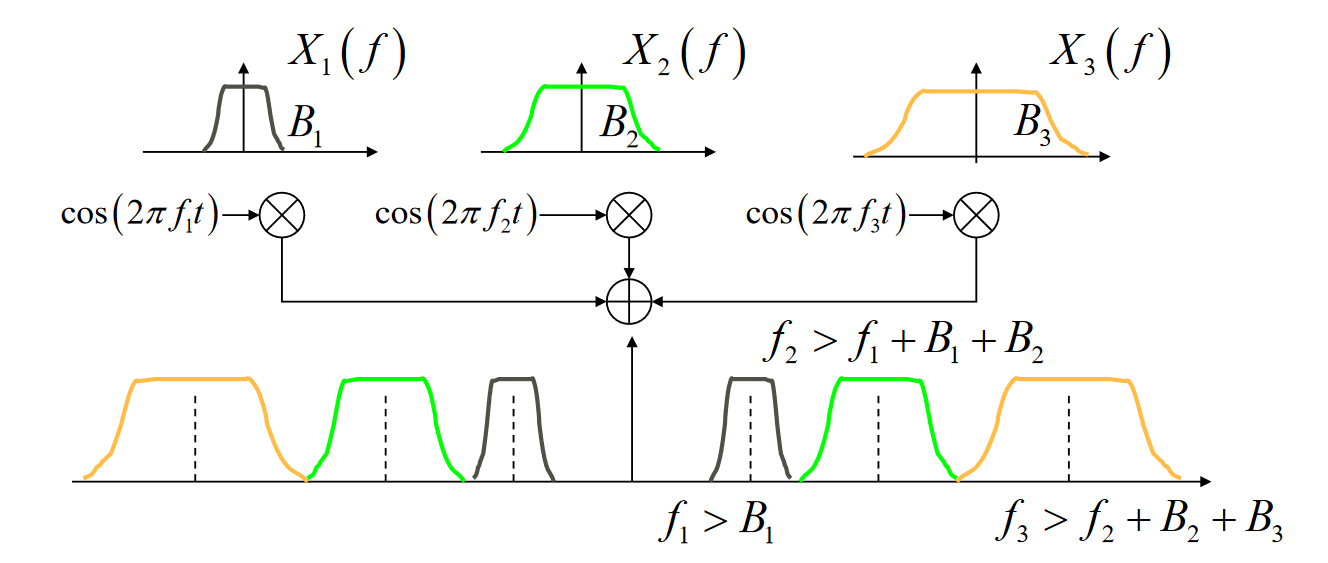
\includegraphics[width=0.9\textwidth]{img/wireless/FDM.png}
        \caption{Frequency Multiplexing}
        \label{fig:FDM}
      \end{figure}
    \end{subsection}
    \begin{subsection}{Analog-to-Digital Conversion}
      We can now deal with signals, but we still have to convey information.\\
      The informations can be both \textbf{analog} or \textbf{digital}. Usually, transmitting digital
      information is ideal, because it has some advantages, such as error detection and correction,
      and the possibility to compress the information. On the other hand, we still have to convert
      digital information to analog information to be transmitted over the channel, after converting
      it to a stream of bits.\\
      Once the signal is received, it has to be converted back to digital information. To do so,
      first of all the signal it has to be sampled, which can be a lossless operation if the sampling
      frequency is high enough.\\
      After the sampling, the sample has to be quantized, which is the process of converting the
      amplitude of the sample to a digital value at discrete times( because it is a continuous
      time function, which would require an infinite number of digits to represent). Each of those 
      values is associated with a given amplitude, which is associated to a number, which 
      eventually is converted into binary digits. We can also observe that quantization is a lossy
      operation by definition.\\
      At the end of the fair, a sequence of bits is obtained, which can be transmitted over the
      channel.\\
      \begin{figure}[h]
        \centering
        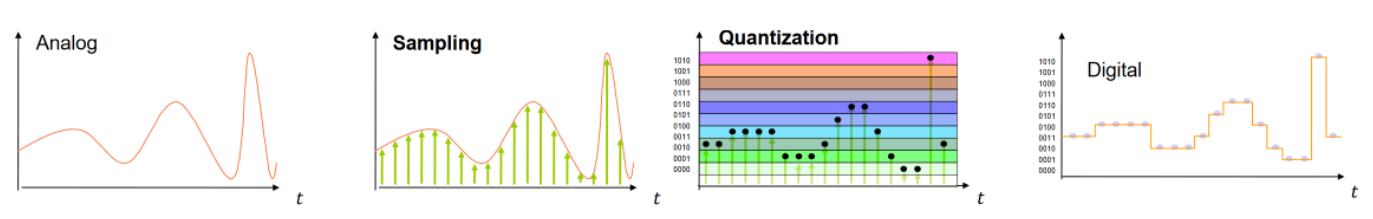
\includegraphics[width=\textwidth]{img/wireless/analog to digital.png}
        \caption{Analog-to-Digital Conversion}
        \label{fig:ADC}
      \end{figure}
      \begin{subsubsection}{Sampling theorem}
        As previously stated, the sampling operation can be lossless if the sampling frequency is
        high enough. This is because of the \textbf{Nyquist sampling theorem}, which states
        that a signal can be perfectly reconstructed from its samples if the sampling frequency is
        at least twice the bandwidth of the signal.\\
        \begin{equation}
          f_c=\frac{1}{T_c}>2B\to T_c<\frac{1}{2B}
        \end{equation}
        where $f_c$ is the sampling frequency, $T_c$ is the sampling period, and $B$ is the bandwidth.
        \end{subsubsection}
    \end{subsection}
\end{section}

\begin{section}{Signal Transmission and Reception}
  Now that we know how a signal can be represented and processed, we can start to think how each 
  component of a communication system can be designed.\\
  \begin{subsection}{Digital Modulations}
    The end goal is to have a reliable communication system, which can transmit and receive
    information. As such, a important design choose is the signal waveform to transmit.\\
    The \textbf{modulator} is the component of the system that takes the digital information and 
    modulates it to a signal that can be transmitted over the channel. The demodulator component 
    just does the opposite, taking the signal and converting it back to digital information.\\

    \begin{boxH}
      \textbf{Modulation} is the process of varying one or more properties of a periodic waveform, called
      the \textbf{carrier}, with a modulating signal that typically contains information to be
      transmitted.
    \end{boxH}
    This process is necessary not only to cope with the analog channel, but also to allow multiple
    communication systems( which means different signals) to coexist in the same channel.\\

    Generally, digital and analog modulations resort to basic modulation types:
    \begin{itemize}
      \item \textbf{Amplitude Modulation(AM)}, which changes the amplitude of the carrier
      \item \textbf{Frequency Modulation(FM)}, which changes the frequency of the carrier
      \item \textbf{Phase Modulation(PM)}, which changes the phase of the carrier
    \end{itemize}

    This kind of modulation is necessary to convey information to the receiver, assigning to each
    possible value of the information signal a different amplitude, frequency or phase.
    \begin{subsubsection}{Amplitude Modulation(AM)}
      The amplitude modulation is the simplest form of modulation.\\
      The amplitude of an high-carrier signal(like a cosine signal) is varied according to the 
      instantaneous amplitude of the modulating message signal $m(t)$.\\
    \end{subsubsection}
    \begin{subsubsection}{Frequency Modulation(FM)}
      In frequency modulation, the frequency of the carrier signal is varied by the modulating
      signal $m(t)$, while the amplitude of the carrier signal is kept constant.\\
      This means that the as the amplitude of the information signal varies, the carrier frequency
      varies as well. For example, if the amplitude of the information signal increases, the
      frequency of the carrier signal increases as well.\\
      \begin{figure}[h]
        \centering
        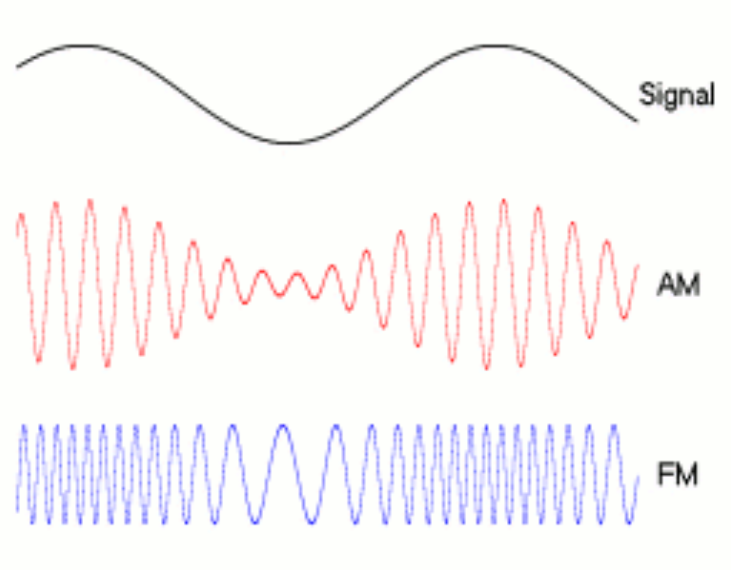
\includegraphics[width=0.4\textwidth]{img/wireless/AM-FM.png}
        \caption{An example of a signal modulated in amplitude and frequency}
        \label{fig:AM-FM}
      \end{figure}
    \end{subsubsection}
    \begin{subsubsection}{Phase Modulation(PM)}
      Phase modulation is a form of modulation that encodes the signal $m(t)$ as a variation in the
      instantaneous phase of a carrier wave.\\
      This means that the phase of a carrier is modulated to follow the changing in the signal 
      amplitude of the message signal.\\

      The peak amplitude and the frequency of the carrier signal are maintained constant, but as 
      the amplitude of the message signal changes, the phase of the carrier changes 
      correspondingly.\\
      \begin{figure}[h]
        \centering
        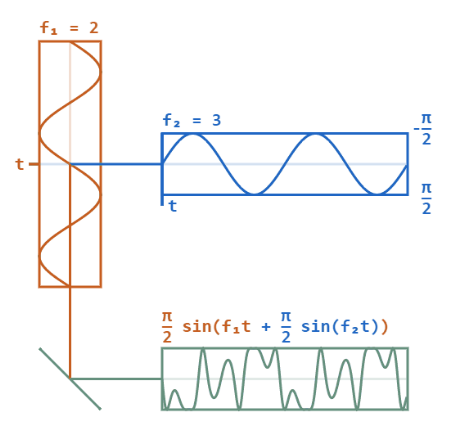
\includegraphics[width=0.5\textwidth]{img/wireless/PM.png}
        \caption{An example of a signal modulated in phase. The modulating wave(in blue) is modulating
          the phase of the carrier wave(in red), resulting in the PM signal(in green)}
        \label{fig:PM}
      \end{figure}
    \end{subsubsection}
    \begin{subsubsection}{Analog-to-Digital modulations}
      Even if the world has turned to digital, transmitted signals are analog.\\
      This means that the digital information has to be converted to an analog signal to be
      transmitted over the channel. But the receiver still need to understand the digital information
      from the received signal.\\
      To be sure that the information can be recovered, the signal has to be modulated in a way that
      the receiver can understand the digital information. This can be done by varying some proprieties
      of the carrier signal, such as the amplitude, the frequency, or the phase, to represent the
      digital information.\\
      \begin{figure}[h]
        \centering
        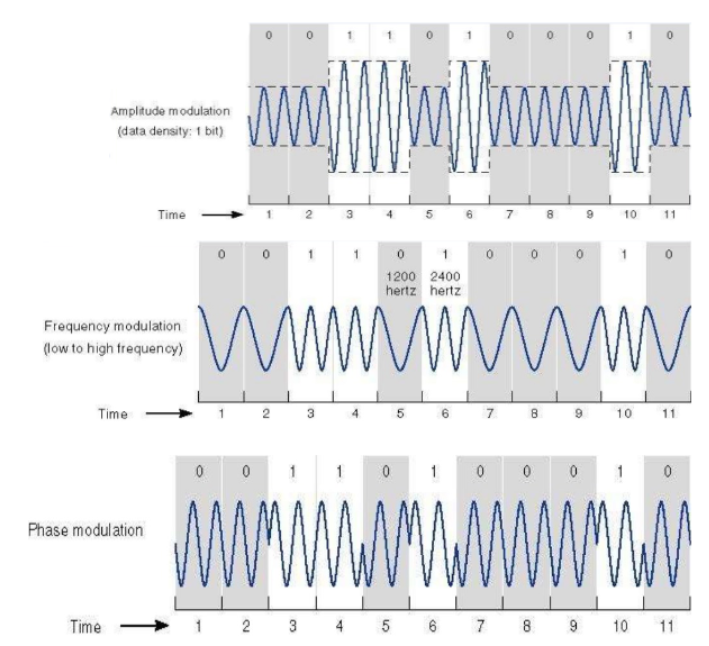
\includegraphics[width=0.5\textwidth]{img/wireless/modulation encoding.png}
        \caption{Some example of modulations used to represent digital information. From top to bottom:
          Amplitude Shift Keying, Frequency Shift Keying, Phase Shift Keying}
        \label{fig:DigitalModulation}
      \end{figure}
      The carrier signal is used to modulate the digital information, so we can distinguish between
      different kinds of signals:
      \begin{itemize}
        \item the \textbf{the baseband signal}, which is the unmodulated signal, whose spectrum is
          centered around zero frequency
        \item the \textbf{passband signal}, which is the modulated signal, whose spectrum is centered
          around the carrier frequency
      \end{itemize}
      The baseband signal can be converted to a passband signal by multiplying it by a carrier signal
      with the desired frequency.\\
    \end{subsubsection}
    \begin{subsubsection}{Baseband Signals}
      The simplest kind of digital modulation is the \textbf{Pulse Amplitude Modulation(PAM)}, which
      is a form of modulation where the message signal is encoded in the amplitude of a series of
      signal pulses.\\
      For example, if we have a binary signal, we can encode the 0 as a low amplitude pulse $-A$, and the
      1 as a high amplitude pulse $A$. The simplest pulse is a rectangular one, but other kind of 
      pulses can be used.\\
      If we have a binary PAM(2-PAM), the signal can be represented as:
      \begin{itemize}
        \item $s(t)=g(t) \to "1"$
        \item $s(t)=-g(t) \to "0"$
      \end{itemize}
      where $g(t)$ is the basic pulse shape.\\
      \begin{figure}[h]
        \centering
        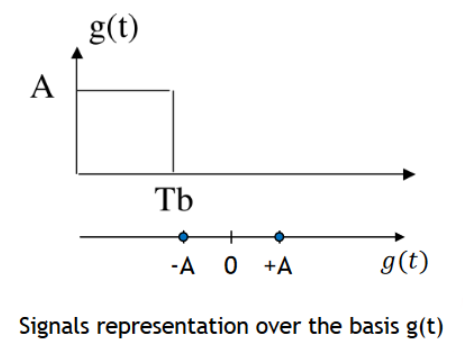
\includegraphics[width=0.4\textwidth]{img/wireless/2-PAM.png}
        \caption{An example of a 2-PAM signal representation}
        \label{fig:PAM}
      \end{figure}
    \end{subsubsection}
    \begin{subsubsection}{M-ary PAM}
      WA 2-PAM signal can only represent 1 bit of information. To represent more bits, we can use
      M-ary PAM, where M is the number of different symbols that can be represented, while still
      using the same base signal.\\
      For example, a 4-PAM signal can represent 2 bits of information by defining 4 levels of
      amplitude, and can be represented as:
      \begin{itemize}
        \item $s(t)=3g(t) \to "00"$
        \item $s(t)=g(t) \to "01"$
        \item $s(t)=-g(t) \to "10"$
        \item $s(t)=-3g(t) \to "11"$
      \end{itemize}
      This definition can be generalized to:
      \begin{equation}
        s_i(t)=A_i g(t),\quad i=1,2,\dots,M
      \end{equation}
      allowing to represent $log_2(M)$ bits of information.\\
      \begin{figure}[h]
        \centering
        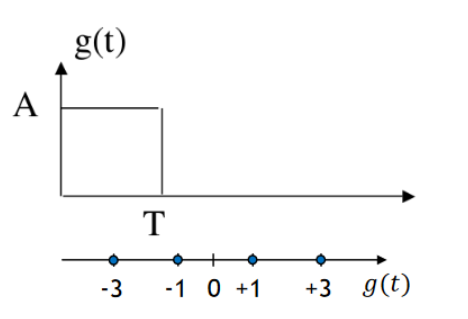
\includegraphics[width=0.4\textwidth]{img/wireless/M-PAM.png}
        \caption{An example of a 4-PAM signal representation}
        \label{fig:4-PAM}
      \end{figure}
    \end{subsubsection}
    \begin{subsubsection}{Gray Coding}
      When using M-ary PAM, it is important to use a coding that minimizes the error probability.
      After all, Symbols that are close to each other in the signal space are more likely to be 
      confused, so the choice of the number of symbols and the distance between them is 
      important.\\
      \begin{boxH}
        \textbf{Gray coding} is a strategy to \textbf{mapping bits to symbols} that minimizes the
        probability of error.
      \end{boxH}
      Gray coding achieves 1-bit error correction, meaning that if a error is to occur, it will only
      affect 1 bit of the message with a high probability.\\
      \begin{figure}[h]
        \centering
        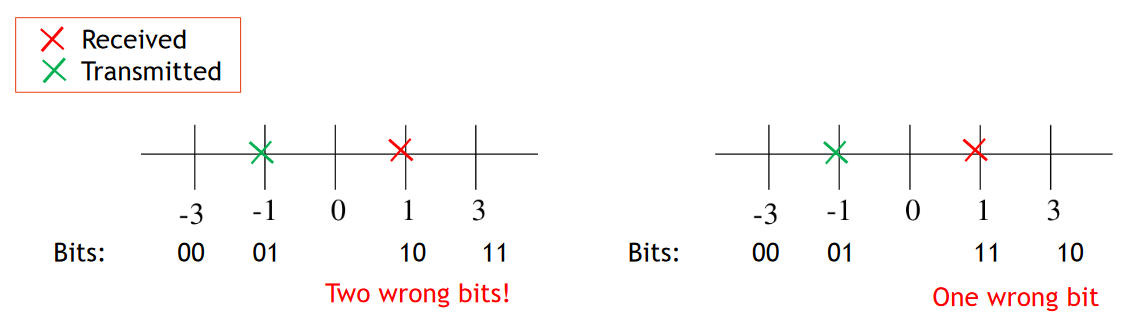
\includegraphics[width=0.8\textwidth]{img/wireless/gray coding.png}
        \caption{An example of a 4-PAM signal representation using Gray coding}
        \label{fig:GrayCode}
      \end{figure}
    \end{subsubsection}
    \begin{subsubsection}{Energy per bit}
      A measure of the energy efficiency of a modulation can be obtained by calculating the average
      energy per bit.\\
      The energy per bit can be defined as 
      \begin{equation}
        E_b=\frac{E_s}{log_2(M)}
      \end{equation}
      where $E_s$ is the energy of the signal, and $M$ is the number of symbols, or in a more
      discursive way, the average energy per symbol divided by the number of bits carried by 
      each symbol.\\
      This concept can also be visualized graphically, as the distance of a symbol from the origin
      in the signal space(as in figure \ref{fig:4-PAM}), because it is proportional to 
      energy of the symbol.\\

      The energy per symbol can be calculated as
      \begin{equation}
        E_s=\int_{0}^{T} (S_m(t))^2 dt= (A_m)^2 \int_{0}^{T} (g(t))^2 dt= (A_m)^2 E_g
      \end{equation}
      where $S_m(t)$ is the modulated signal, $A_m$ is the amplitude of the modulated signal, $g(t)$
      is the base pulse, and $E_g$ is the energy of the base pulse.\\

      For example, the average energy per symbol for the 4-PAM of figure \ref{fig:4-PAM} is
      \begin{equation}
        E_s=\frac{3^2T+1^2T+1^2T+3^2T}{4}=5T
      \end{equation}
      Generally, the larger the energy, the larger the distance between the symbols, and the lower
      the probability of error(mistaking one symbol for another). On the other hand, the larger the
      number of symbols over the same bandwidth, the less energy is required to transmit each bit(
      because each symbol is closer and carries more bits).\\
    \end{subsubsection}

    \begin{subsubsection}{Bandpass Signals}
      As previously stated, to transmit a baseband signal $s(t)$ trough a passband channel, we 
      have to modulate it at a certain frequency $f_c$, by multiplying it by a sinusoidal carrier
      signal with that frequency, otherwise it will be centered around zero frequency.\\
    \end{subsubsection}

    \begin{subsubsection}{Bandwidth Occupancy and efficiency}
      The shape of a signal determine the bandwidth it occupies.\\
      For example, a rectangular function has a pulse spectrum that is a sinc function, shown in
      figure \ref{fig:rectangular pulse spectrum}, which has a symbol rate of $1/T$(the amount of 
      symbols per second).

      \begin{figure}[h]
        \centering
        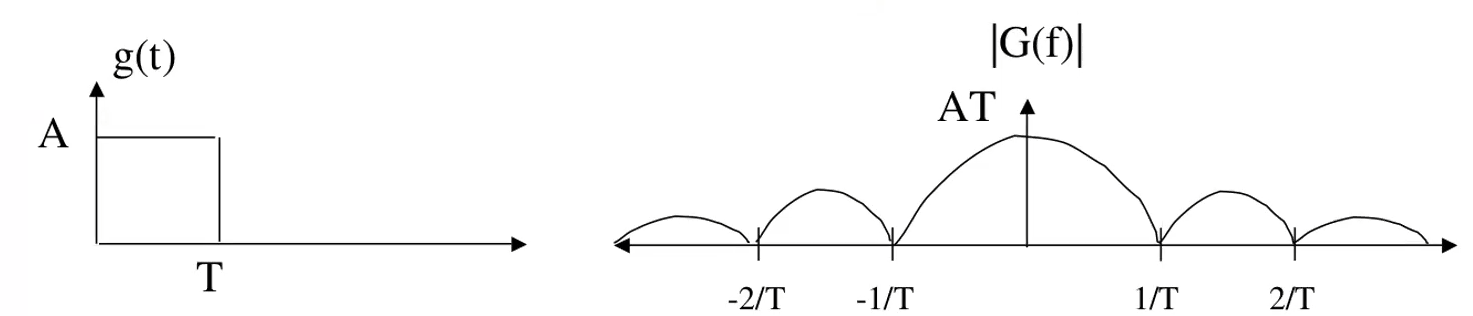
\includegraphics[width=0.6\textwidth]{img/wireless/rectangular pulse spectrum.png}
        \caption{The spectrum of a rectangular pulse}
        \label{fig:rectangular pulse spectrum}
      \end{figure}

      Usually, a smaller base pulse will require less energy to transmit, but will occupy more
      bandwidth. A longer basic pulse will require more energy to transmit, but will occupy less
      bandwidth and have a lower bit rate.\\

      With that in mind, ideally, we would like to choose a pulse shape $g(t)$ that minimizes the
      bandwidth occupancy, putting more energy in the lower frequencies, resulting in a smaller
      bandwidth.\\

      For a pulse duration $T$, we can define the \textbf{symbol rate} as $R_s=1/T$, and the
      \textbf{bit rate} as $R_b=R_s log_2(M)$(recall that $log_2(M)$ is the number of bits per
      symbol).\\
      The bit rate efficiency can be defined as
      \begin{equation}
        \eta=\frac{R_b}{BW}=\frac{log_2(M)}{T} \times (\frac{T}{2})=\frac{log_2(M)}{2}\text{bps/Hz}
      \end{equation}
      where $BW$ is the two sided bandwidth of the signal $BW=2R_2=\frac{2}{T}$.\\
      As we can see, the bit rate efficiency is proportional to the number of bits per symbol
      ($\eta \propto M$) and inversely proportional to the pulse duration. The duration of the 
      pulse is uninfluent.\\

      We can also consider some examples:
      \begin{itemize}
        \item 2-PAM: $\eta=\frac{1}{2}\text{bps/Hz}$
        \item 4-PAM: $\eta=\frac{2}{2}\text{bps/Hz}$
        \item 8-PAM: $\eta=\frac{3}{2}\text{bps/Hz}$
      \end{itemize}
      As we can see, the bandwidth efficiency increases with the number of bits per symbol, because
      we are fitting more bits in the same bandwidth.\\
      This also means that our signal will be more susceptible to noise, because the symbols are
      closer to each other, making it easier to mistake one for another. To reduce the probability
      of errors, we have to increase the energy per symbol, which will increase the bandwidth
      occupancy. For those reasons, there's a trade-off between bandwidth occupancy and energy
      efficiency.\\

      \begin{figure}[h]
        \centering
        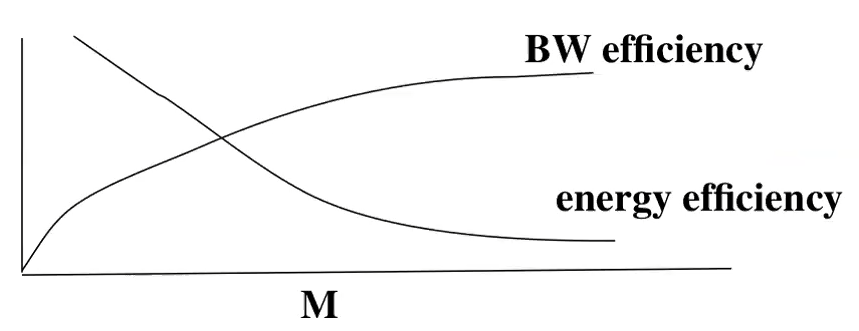
\includegraphics[width=0.6\textwidth]{img/wireless/energy efficiency vs bandwidth occupancy.png}
        \caption{Trade-off between energy efficiency and bandwidth occupancy}
        \label{fig:energy efficiency vs bandwidth occupancy}
      \end{figure}

    \end{subsubsection}
    \begin{subsubsection}{Two-dimensional Modulation}
      As introduced in subsection \ref{sub:IQ representation}, signals can be represented over two 
      orthonormal basis. This means that we can represent a signal in a 2D plane, with the
      in-phase and quadrature components as the x and y axis.\\
      This representation allows to represent the set of signals $s_i$(also called \textit{constellation}
      over two orthonormal basis. A large constellation will allow to represent more bits per symbol,
      which results in a higher bit rate(bandwidth efficiency), but also a higher probability of 
      error.\\

      \begin{boxH}
        The shape of the constellation is important, because it can be used to minimize the probability
        of error, by choosing a constellation that minimizes the distance between the symbols.
      \end{boxH}
      \begin{figure}[h]
        \centering
        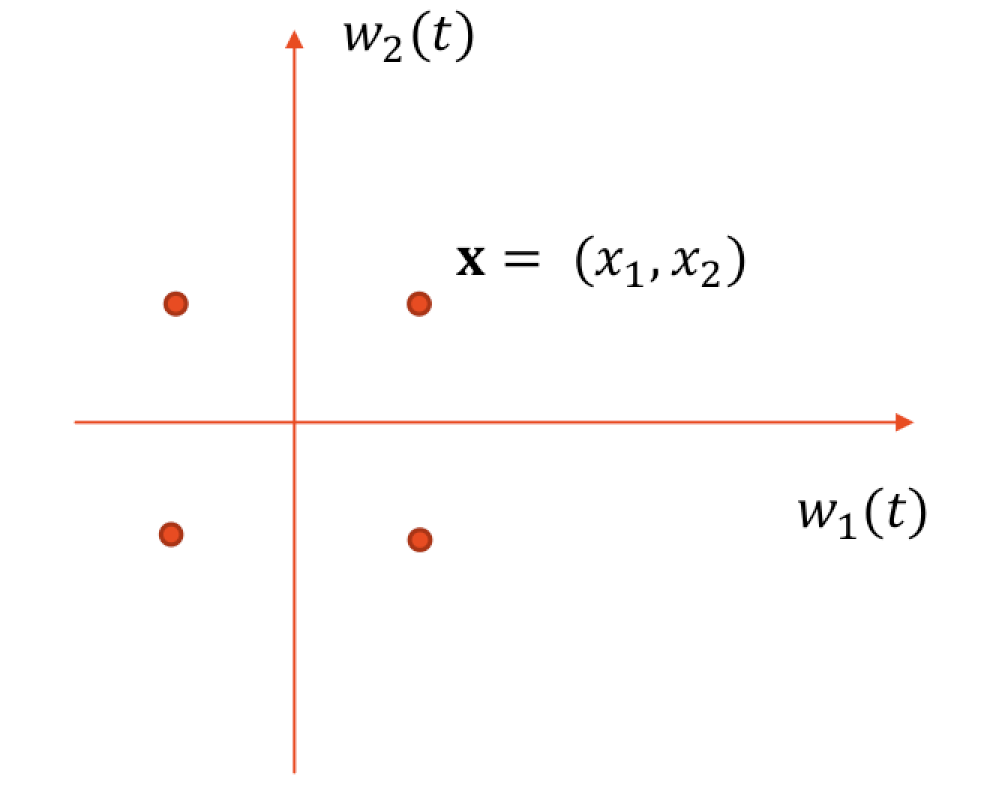
\includegraphics[width=0.5\textwidth]{img/wireless/iq representation.png}
        \caption{A constellation of 4-PAM signals}
      \end{figure}
      Furthermore, there are some common constellations that are used in practice, such as:
      \begin{itemize}
        \item \textbf{QAM}: Quadrature Amplitude Modulation, which is a PAM signal over two
          dimensions.
        \item \textbf{PSK}: Phase Shift Keying, which is a PAM signal over the phase of a signal, 
          meaning that the amplitude is constant.
      \end{itemize}
    \end{subsubsection}

    \begin{subsubsection}{M-QAM}
      \begin{boxH}
        M-QAM is a modulation that represents the signal as the sum of two signals, represented over
        two orthonormal basis. This means that we can have $M$ symbols to modulate out signal.
      \end{boxH}
      Thus, we can represent $\sqrt{M}$ symbols over each axis, and the total number of
      symbols is $M$.\\
      This means that a symbol, represented over two orthonormal basis, can be described as 
      \begin{equation*}
        S_m=(A^x_m,A^y_m),A^x_m,A^y_m \in \{+/-1,\dots,+/-(\sqrt{M}-1)\}
      \end{equation*}
      for example:
      \begin{itemize}
        \item 4-QAM: $A^x_m,A^y_m \in \{+/-1\}$
        \item 16-QAM: $A^x_m,A^y_m \in \{+/-1,+/-3\}$
      \end{itemize}

      \begin{figure}[h]
        \centering
        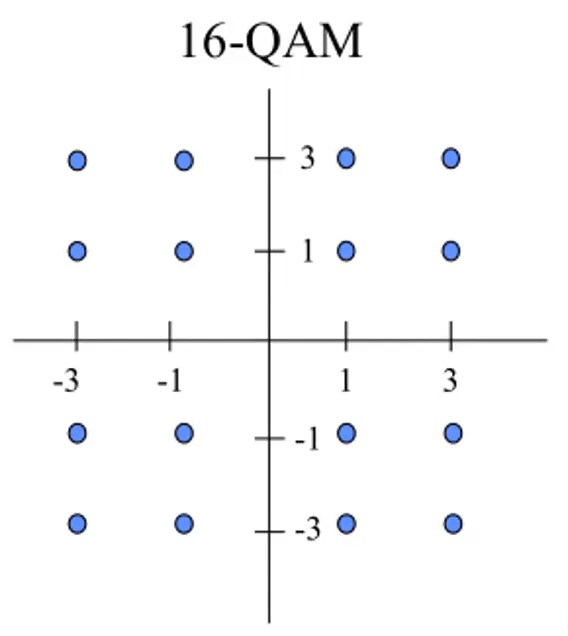
\includegraphics[width=0.4\textwidth]{img/wireless/16 QAM.png}
        \caption{A 16-QAM constellation}
      \end{figure}

      We recall that with QAM, the amplitude and phase of the signal are modulated. This means that
      by using the same pulse shape $g(t)$, the bandwidth efficiency is the same of a M-PAM, because
      the number of bits per symbol is the same, but with a larger energy efficiency, thanks to the
      presence of another dimension.\\

      By entering in the details, the in-phase and quadrature components of the signal are modulated
      by multiplying the components to orthogonal carriers, meaning that we can separate them 
      easily afterwards. This operation also transform the signal to a bandpass one.\\
      This is accomplished by multiplying the $A^x$ component by Cosine and the $A^y$ component by
      Sine, and then summing the two signals.\\

      The transmitted signal can thus be described as
      \begin{equation}
        U_m(t)= A_m^xg(t)cos(2\pi f_c t)+A_m^yg(t)sin(2\pi f_c t),m=1,\dots,M
      \end{equation}
      or in a more discursive way, each component of the signal is the amplitude value over one axis
      multiplied by the base pulse(the basis), and then multiplied by a carrier signal at a 
      given frequency.\\
    \end{subsubsection}
    \begin{subsubsection}{M-QAM modulation and demodulation}
      The general schema of M-QAM modulation is shown in figure \ref{fig:MQAM modulation}.\\
      We receive in input a series of bits, which are associated with the corresponding symbols, 
      one for each axis. The symbols used to modulate the pulse signal are then multiplied by the
      pulse shape, and then by the carrier signal. The two signals are then summed and transmitted.\\

      \begin{figure}[h]
        \centering
        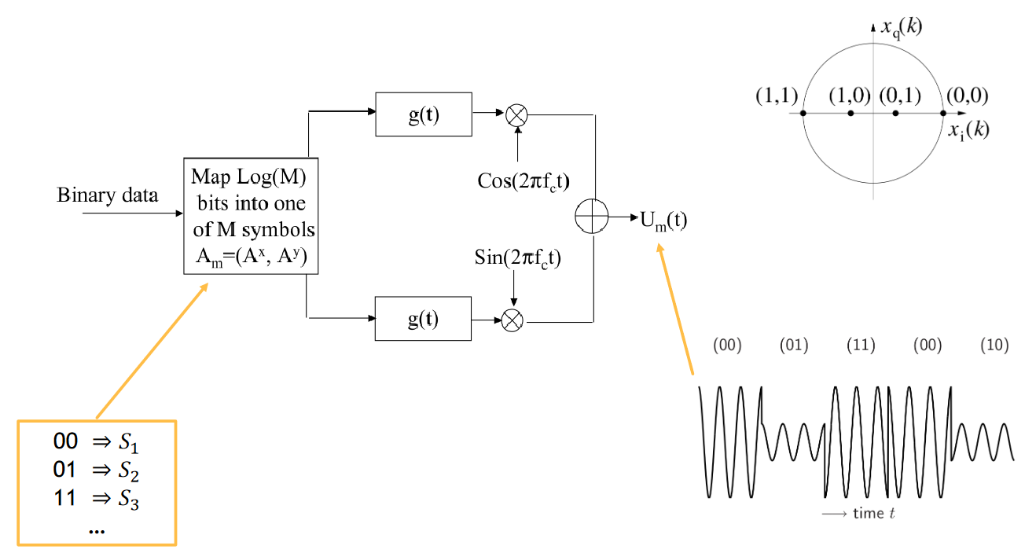
\includegraphics[width=0.7\textwidth]{img/wireless/MQAM modulation.png}
        \caption{General schema of M-QAM modulation}
        \label{fig:MQAM modulation}
      \end{figure}

      As for what concerns the demodulation, we want to understand correctly the symbols that we
      receive, so we don't really care about the carrier signal. 
      We can notice that the sin and cosine components of the signal are orthogonal, meaning that
      we are able to separate them easily: the cosine component disappears after filtering when multiplied
      by the sine component, and viceversa.\\
      \begin{figure}[h]
        \centering
        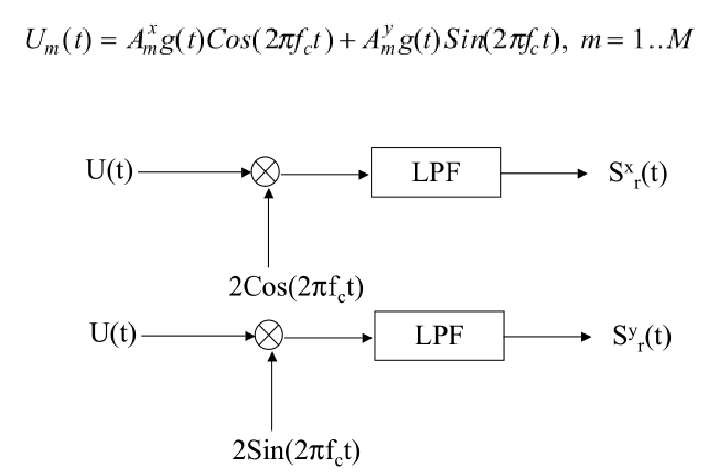
\includegraphics[width=0.5\textwidth]{img/wireless/MQAM demodulation.png}
        \caption{General schema of M-QAM demodulation}
        \label{fig:MQAM demodulation}
      \end{figure}
    \end{subsubsection}
    \begin{subsubsection}{Phase Shift Keying}
      \begin{boxH}
        \textbf{Phase Shift Keying}(PSK) is a PAM signal over the phase of a signal.\\
        In a PSK constellation, the amplitude of the signal is constant, meaning that
        all the signals have the same energy.
      \end{boxH}

      This means that the symbols are equally spaced across a circle of radius $\sqrt{E_S}$, where
      $E_S$ is the energy of the signal.\\
      Symbols are thus equally spaced to minimize the probability of error.\\

      \begin{figure}[h]
        \centering
        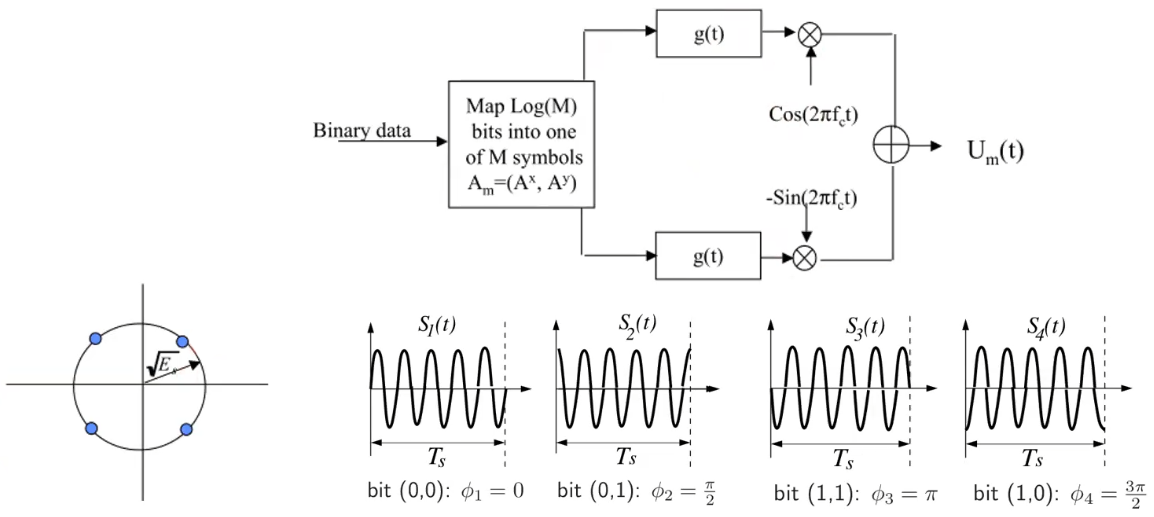
\includegraphics[width=0.7\textwidth]{img/wireless/MPSK modulation.png}
        \caption{General schema of M-PSK modulation}
        \label{fig:MPSK modulation}
      \end{figure}
      The modulation process is similar to the one of M-QAM. We can notice that, because all the 
      amplitude values are so similar, resulting the waveforms have the same energy.
    \end{subsubsection}

    \begin{subsubsection}{Power amplifiers}
      After modulation, the signal is usually amplified by a \textbf{power amplifier} to increase
      the power of the signal.\\
      \begin{figure}[h]
        \centering
        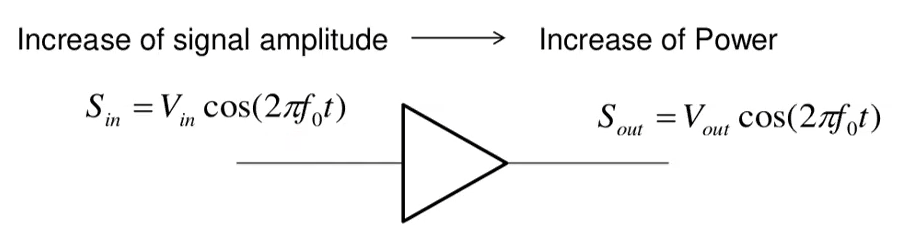
\includegraphics[width=0.5\textwidth]{img/wireless/power amplifier.png}
        \caption{General schema of a power amplifier}
        \label{fig:power amplifier}
      \end{figure}
      Because we cannot have infinite energy, we can only amplify the signal to a certain level, 
      which is called \textbf{saturation level}.\\
      This has some effect on the constellations of a signals:
      \begin{itemize}
        \item when working with \textbf{PSK} signals, the constellation in amplified uniformly
          even when working in saturation.
        \item when working with \textbf{QAM} signals, the constellation is scaled differently, 
          making the probability of error higher.
      \end{itemize}

      \begin{figure}[h]
        \centering
        \subfloat[PSK constellation after amplification]{
          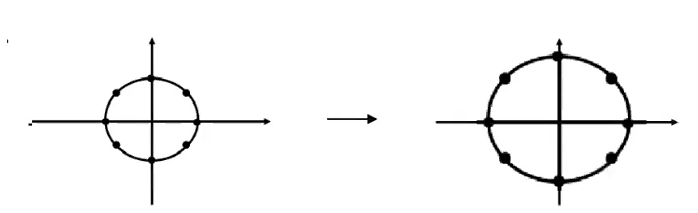
\includegraphics[width=0.4\textwidth]{img/wireless/PSK amplification.png}
          \label{fig:PSK amplification}
      }
        \hfill
        \subfloat[QAM constellation after amplification]{
          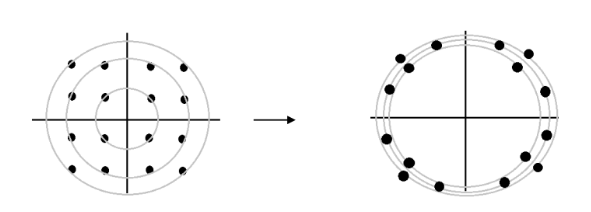
\includegraphics[width=0.4\textwidth]{img/wireless/QAM amplification.png}
          \label{fig:QAM amplification}
      }
        \caption{Effect of power amplification on a signal}
        \label{fig:constellation after amplification}
      \end{figure}
      When working under the saturation level, the power amplifier is linear, meaning that the
      output signal is proportional to the input signal, and no distortion occurs, but the 
      amplifier is underexploited.\\
      Thus, there is a trade-off between transmitted power and signal quality.\\
      
    \end{subsubsection}
  \end{subsection}

  \begin{subsection}{AWGN channel and equalization}
    Recall that to transmit information, we need to send a signal over a channel, in our case a 
    wireless one.\\
    We already briefly discussed the disturbance of a signals in subsection \ref{subsec:channel}, but the 
    main challenges can be summarized as:
    \begin{itemize}
      \item share the medium via \textbf{multiplexing}
      \item fight \textbf{noise} and \textbf{channel impairments}
    \end{itemize}
    The major sources of errors in the channel are essentualy two:
    \begin{itemize}
      \item \textbf{Termal noise}(AWGN), which is the result of the thermal agitation of the electrons
        in the receiver. It disturbs the signal in an additive fashion and occupies all the
        frequency band. Is also modelled by a Gaussian random process.
      \item \textbf{Inter-Symbol Interference}(ISI), which is the result of the signal being reflected
        by obstacles, and thus arriving at the receiver with a different phase and amplitude.
    \end{itemize}
    \begin{figure}[h]
      \centering
      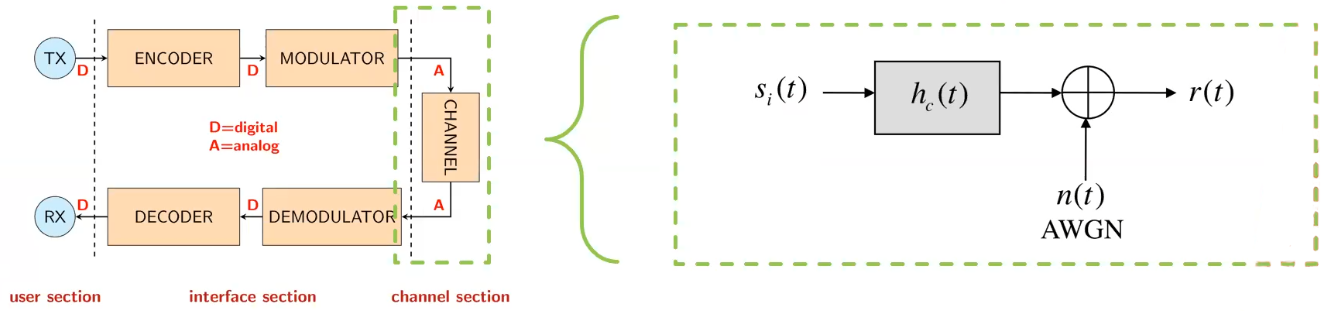
\includegraphics[width=0.8\textwidth]{img/wireless/channel effect.png}
      \caption{Effects of the channel on a signal, $h(t)$ is a filter that models the channel with it impusle response,
        and $n(t)$ is the noise}
      \label{fig:channel effects}
    \end{figure}
    We can say that the channel ruin the signal. This is evident when looking at the spectrum of the
    signal, which is spread by the channel, shown in figure \ref{fig:channel effect on the spectrum}.\\
    \begin{figure}[h]
      \
      \centering
      \subfloat[Effect of the noise on the signal]{
        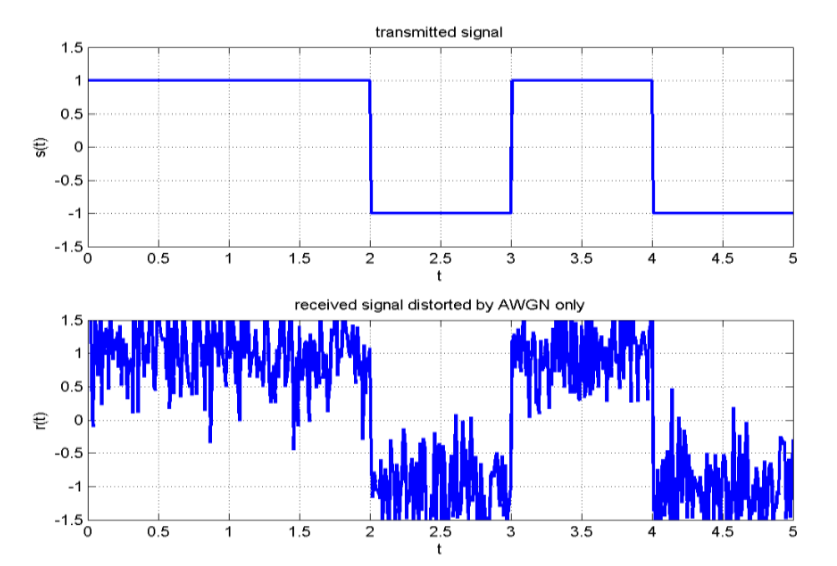
\includegraphics[width=0.4\textwidth]{img/wireless/signal AWGN effect.png}
        \label{fig:signal AWGN effect}
      }
      \hfill
      \subfloat[Signal spectrum distorted by inter-symbol interference, modelled by $h_c(t)$]{
        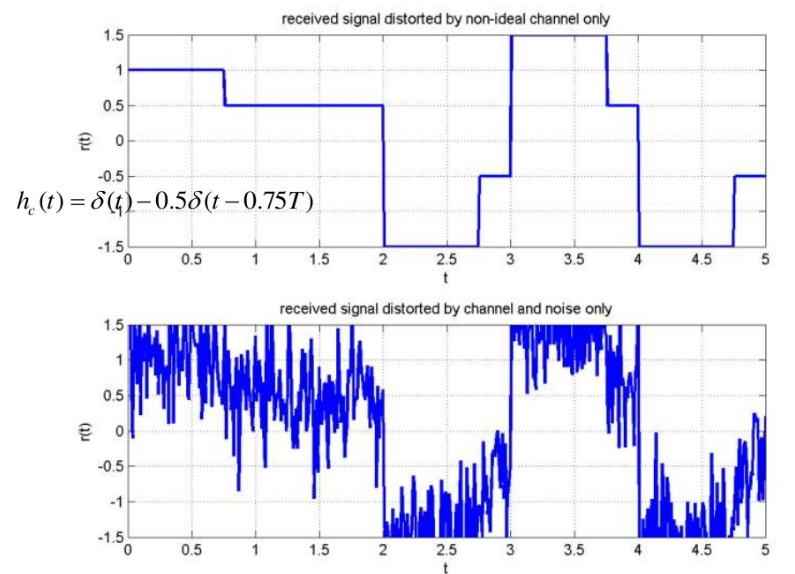
\includegraphics[width=0.4\textwidth]{img/wireless/signal filter effect.png}
        \label{fig:signal spectrum after channel}
      }
      \caption{Effect of the channel on the spectrum of a signal}
      \label{fig:channel effect on the spectrum}
    \end{figure}
    \begin{subsubsection}{Receiver Task}
      We want to design a receiver that can mitigate (or even revert) those two effects, to be 
      able to correctly understand the signal.\\
      To do so, we have to \textbf{demodulate} the signal and \textbf{equalize} it.\\
      This process can be carried out in 3 steps:
      \begin{enumerate}
        \item Improve the signal-to-noise ratio(SNR) using a \textbf{matched filter}
        \item Reduce Inter-Symbol Interference(ISI) using an \textbf{equalizer}
        \item Sample the recovered waveform and guess the transmitted symbol
      \end{enumerate}
      After those steps, we still have an imperfect signal wave, so we need to \textbf{detect} the
      transmitted symbol, thresholding the signals to remove outliers introduced in the channel 
      and decide with symbol was transmitted.\\
      \begin{figure}[h]
        \centering
        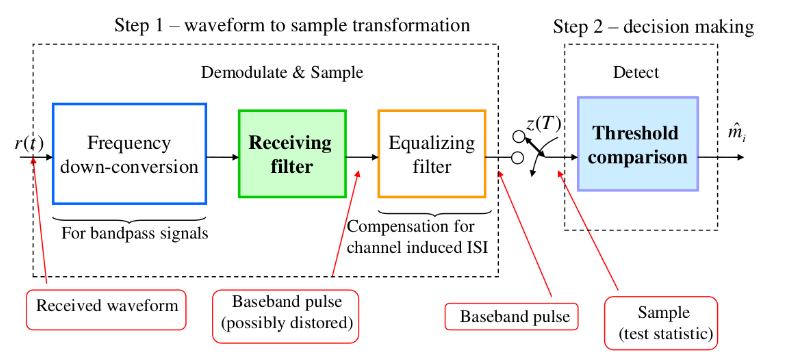
\includegraphics[width=0.8\textwidth]{img/wireless/receiver steps.png}
        \caption{General steps that a receiver has to carry out}
        \label{fig:receiver task}
      \end{figure}
    \end{subsubsection}

    \begin{subsubsection}{Maximize SNR}
      \begin{boxH}
        To maximize the signal-to-noise ratio, we can use a \textbf{matched filter} $h(t)=g(T-t)$
      \end{boxH}
      Turns out that the input response of the optimal filter is the time-reversed version of the
      pulse shape.\\
      The receiver must know the basic pulse shape to be able to use the matched filter.\\
      \begin{figure}[h]
        \centering
        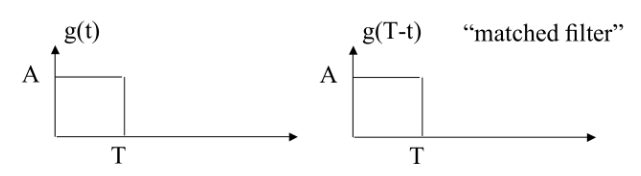
\includegraphics[width=0.6\textwidth]{img/wireless/matched filter.png}
        \caption{Effect of the matched filter on the signal. They are kind of the same because
        the function is symmetrical}
        \label{fig:matched filter}
      \end{figure}
    \end{subsubsection}

    \begin{subsubsection}{Minimize ISI}
      Inter-Symbol Interference is the result  of the filtering effect of the channel, and can be
      defined as 
      \begin{equation}
        H_c(f)=|H_c(f)|e^{j\phi_c(f)}
      \end{equation}
      where $|H_c(f)|$ is the amplitude response of the channel, which is non-constant meaning 
      that it distorts the amplitude of the signal, and $\phi_c(f)$ is the phase response of the
      channel, which is non-linear, meaning that it distorts the phase of the signal.\\

      To revert those effects, we can use an \textbf{equalizer} to compensate for the distortion
      of the channel, which ideally would be the inverse of the channel($H_e(f)=\frac{1}{H_c(f)}$).\\
      Applying it to the signal allows us to get an approximation of the original symbol that was
      transmitted $\hat{S_i}(t)$.\\

      To build the equalizer we still need to know the frequency response of the channel.
      To do that, we can try to estimate the channel based on known characteristics of the signal.
      Usually we don't know them, so we introduce \textbf{pilot symbols} in the signal, which are
      known signals to the receiver, and can be used to estimate the channel.
    \end{subsubsection}

    \begin{subsubsection}{Fading}
      Depending on the channel, its impulse response can vary very slowly or very quickly.\\
      When the impulse response varies slowly, we talk about \textbf{slow fading}, and when it
      varies quickly, we talk about \textbf{fast fading}.\\
      Depending on this, pilots symbols may need to be transmitted more or less frequently.\\
      \begin{figure}[h]
        \centering
        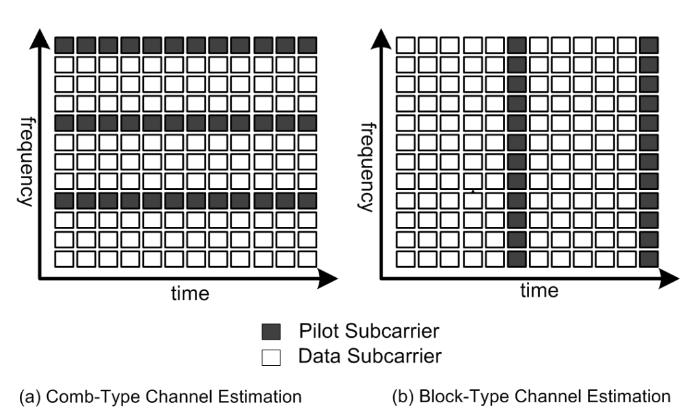
\includegraphics[width=0.6\textwidth]{img/wireless/pilot transmission scheme.png}
        \caption{Pilot transmission scheme}
        \label{fig:pilot transmission}
      \end{figure}
    \end{subsubsection}
  \end{subsection}
  \begin{subsection}{Received symbols and decision regions}
    After equalizing the signal, we would like to decide which symbol was transmitted.\\
    As previously stated, we get a set of possible symbols $S_m\in\{S_1,S_2,...,S_M\}$, and we
    want to decide which one was transmitted, adopting a statistical approach.\\
    \begin{subsubsection}{Symbol Detection}
      Mathematically speaking, we have an hypothesis testing problem, which wants to minimize the
      probability of decision error, meaning that we want to choose the symbol that maximizes the
      probability of the received signal given the transmitted symbol.\\
      
      This is known as the \textbf{Maximum a posteriori probability} (MAP) decision rule, which
      simplify that rule. In fact, turns out that maximizing the probability of the received signal
      given the transmitted symbol is equivalent to minimizing the distance between the received
      signal and the transmitted symbol, under certain conditions.\\
      This is also known as \textbf{Minimum distance decoding} $d_{rS_m}=(r-S_m)^2$, where $r$ is the
      received signal(actual value of the signal plus the noise).\\

      Take for example the case of a 2-PAM signal, shown in figure \ref{fig:signal detection example}.
      The noise alter the received signal, so we can define it as $r=S_m+n$, where $n$ is the noise.
      We also know that the noise is a Gaussian random process, so we can suppose that the noise is
      more likely will be zero, and its less likely will be far from it.\\
      This means that it is possible to assume that the received signal $r$ is more likely to be the
      symbol $S_m$ that is actually closer to it.\\
      So, in this case, we can define the decision region as the interval $[-\infty,0)$ and $(0,\infty]$,
      and the decision rule as
      \begin{equation}
        \hat{S_m}=\begin{cases}
          S_1 & \text{if } r<0\\
          S_2 & \text{if } r\geq 0
        \end{cases}
      \end{equation}
      This can also be generalized to the case of M-PAM signals, because the general idea is still valid.
      \begin{figure}[h]
        \centering
        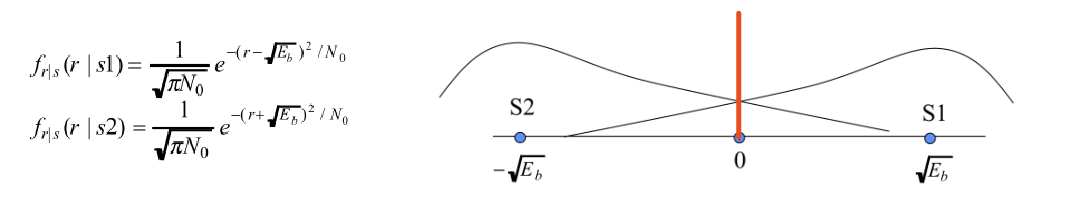
\includegraphics[width=0.8\textwidth]{img/wireless/signal detection example.png}
        \caption{Example of signal detection}
        \label{fig:signal detection example}
      \end{figure}
    \end{subsubsection}
    \begin{subsubsection}{Probability of error}
      The Minimum Distance Decoding rule adopts a statistical approach to decide which symbol was
      transmitted, so it is possible to make errors.\\
      In general, the probability of error $P_e$ between two symbols separated by a distance $d$ is
      \begin{equation}
        P_e=Q\left(\frac{d}{2\sigma}\right)
      \end{equation}
      where $Q$ is a complex function, and $N_0$ is the noise density.\\
      The probability of error can be minimized by increasing the distance between the symbols.

      Based on that we can compute the probability of error per bit, or Bit Error Rate(BER), for 
      each modulation scheme.\\
      Under certain condition, for example grey coding, the BER can be approximated as
      \begin{equation}
        BER=\frac{P_e}{\log_2(M)}
      \end{equation}
      \begin{figure}[h]
        \centering
        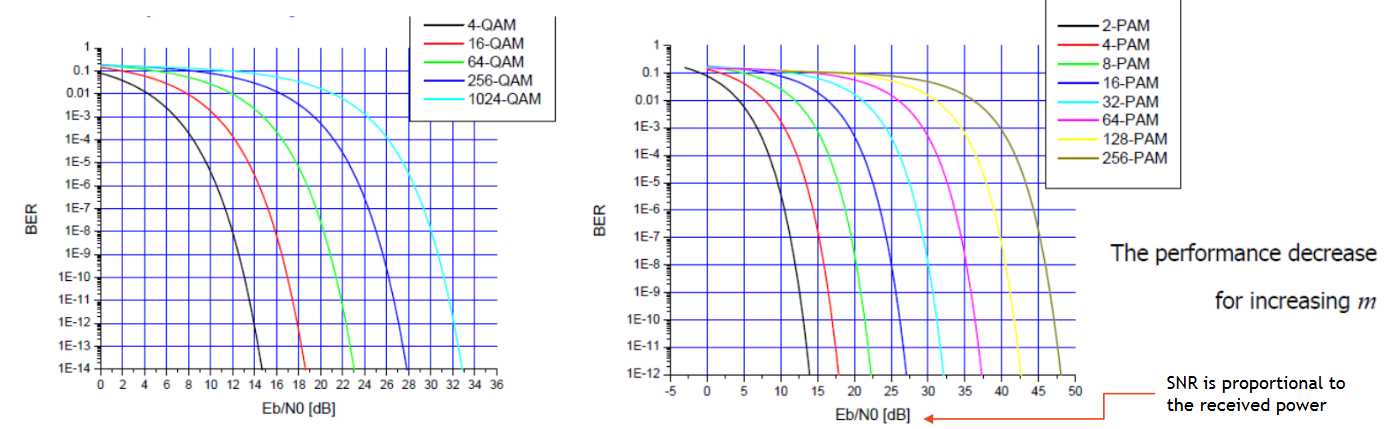
\includegraphics[width=\textwidth]{img/wireless/BER plots.png}
        \caption{Examples of BER plots for different modulation schemes. The BER is higher at the same 
        SNR for denser modulation schemes}
        \label{fig:BER plots}
      \end{figure}
    \end{subsubsection}
  \end{subsection}
  \begin{subsection}{Signal Attenuation and Link Budget}
    During the propagation of a signal, especially in wireless medium, it suffers from an 
    attenuation $L$, which is the loss of power of the signal.\\
    In general, it depends on many environmental factors, such as the distance between the
    transmitter and the receiver, the frequency of the signal, the presence of obstacles, and so on.\\

    The relationship between transmission and reception power is given by the $P_{R}=P_{T}/L$, where
    $P_{R}$ is the received power, $P_{T}$ is the transmitted power, and $L$ is the attenuation.\\
    Given this relationship, we can define the Signal-to-Noise Ratio(SNR) perceived by the receiver
    as
    \begin{equation}
      SNR=\frac{E_b}{N_0}
    \end{equation}
    where $E_b$ the ratio between the Received Power and the Bit Rate, and $N_0$ is the noise density.\\
    In general, to deal with this problem, we use antennas and amplifiers to increase the power of the
    signal and compensate for the attenuation. The shape of the antenna allows to modulate the
    rate of the signal: for example a wider antenna allows to spread the signal in a isotropic way
    and reach a wider area, while a more focused antenna allows to reach a more specific one.\\
    This is measure by the \textbf{beamwidth} of the antenna $\theta_B$, which is a measure of the 
    directivity of the antenna.\\

    \begin{boxH}
      The smaller the beamwidth, the more focused the antenna is, hence we yield a higher gain, but
      we also have a smaller area of coverage.\\
      The larger the beamwidth, the more isotropic the antenna is, hence we yield a lower gain, but
      we also have a larger area of coverage.\\
    \end{boxH}
    For example, a parabolic antenna has a very small beamwidth, so $\theta_B \approx 70\gamma/D$
    where $D$ is the diameter of the antenna.\\
    In general, the gain $G_T$ is proportional to the area of the antenna, so $G_T\propto 1/D^2$.
    Doubling the diameter of the antenna, we get a 4 times increase in the gain.\\

    \begin{figure}[H]
      \centering
      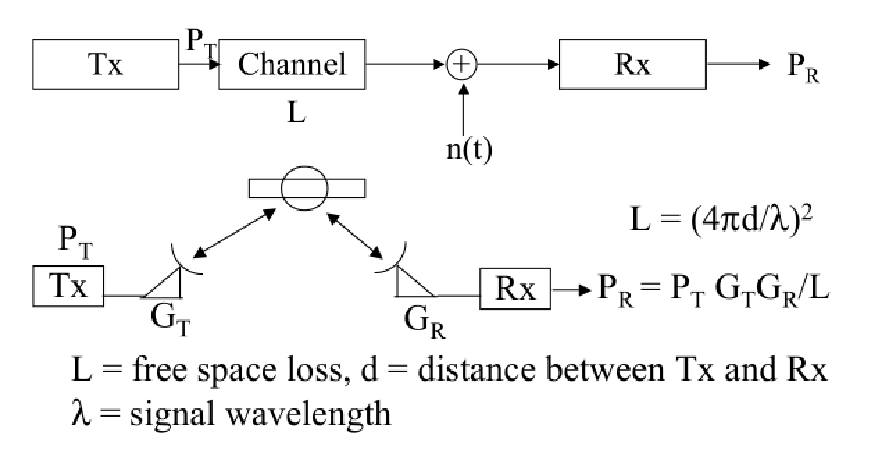
\includegraphics[width=0.6\textwidth]{img/wireless/signal attenuation.png}
      \caption{Example of signal attenuation over a wireless medium}
      \label{fig:antenna gain}
    \end{figure}
  \end{subsection}
  \begin{subsection}{Multiple Access Schemes}
    \begin{boxH}
      As previously discussed in section \ref{subsec:FDM}, we to trasmitt multiple signals over the same
      same shared medium, we have to use a method called \textbf{multiplexing}.
    \end{boxH}
    Multiplexing allows to divide the available bandwidth over multiple logical channels.\\
    The multiplexed signals are then transmitted over the same medium, and then demultiplexed at the
    receiver.\\

    Multiplexing on itself is not enough to allow multiple users to transmit over the same medium.
    We also need to use a method called \textbf{Multiple Access}, which allows multiple users to
    transmit over the same medium.\\
    \begin{boxH}
      \textbf{Multiplexing} deals with \textbf{combining signals}, while \textbf{multiple access} 
      deals with allowing \textbf{multiple users} to access and share a communication medium.
    \end{boxH}
    \begin{subsubsection}{Frequency Division Multiplexing/Multiple Access}
      As previously discussed, FDM allows to divide the available bandwidth over multiple logical
      channels.\\
      In the case of multiple access, we can use FDM to divide the available bandwidth over multiple
      users, and then modulating each user's signal over a different carrier frequency.\\
      This is done by assigning a different frequency band to each user, so that they can transmit
      over the same medium without interfering with each other.\\
      This is the case of \textbf{Frequency Division Multiple Access} (FDM/FDMA).\\
      With this schema, each user get access to the full bandwidth for the whole time, being able to
      completely avoid interference, but if the user is not transmitting, the channel is wasted.\\
      Furthermore, it is necessary to have a guard band between the channels to avoid interference.\\
      \textit{ All wireless systems use this scheme}.
      \begin{figure}[h]
        \centering
        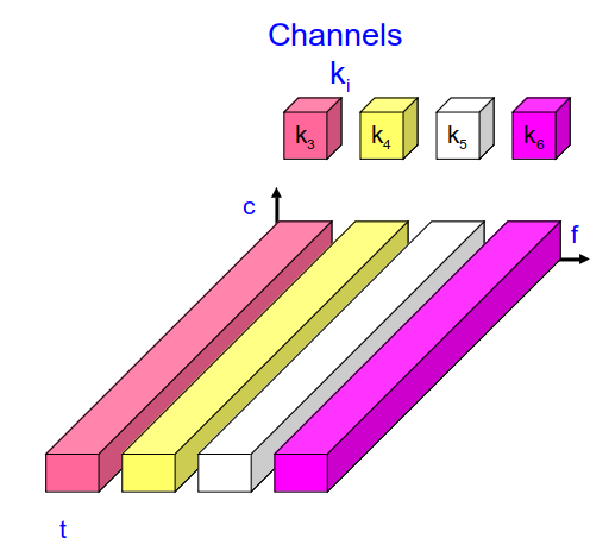
\includegraphics[width=0.4\textwidth]{img/wireless/FDMA.png}
        \caption{Example of FDMA}
        \label{fig:FDMA}
      \end{figure}
    \end{subsubsection}
    \begin{subsubsection}{Time Division Multiplexing/Multiple Access}
      TDM is a method that allows to divide the available bandwidth over multiple logical channels,
      by assigning a different time slot to each user.\\
      This slot is allocated to the user even if it has no data to transmitt. For this method to 
      work correctly some kind of synchronization is needed, but each communication channel has
      access to the full bandwidth, even if it is only for a fraction of the time.\\
      \begin{figure}[h]
        \centering
        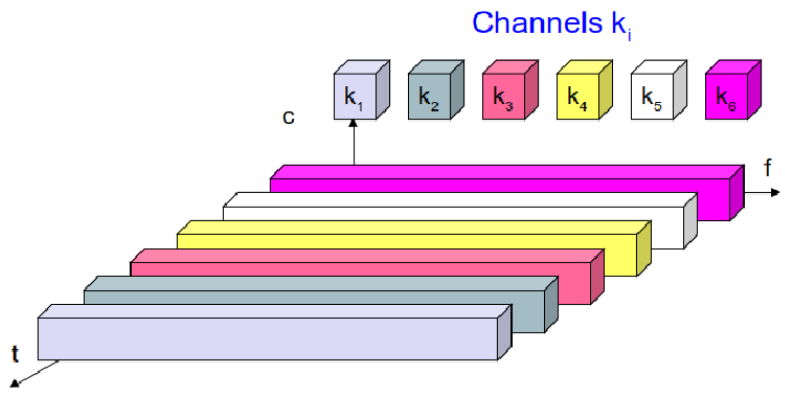
\includegraphics[width=0.4\textwidth]{img/wireless/TDMA.png}
        \caption{Example of TDMA}
        \label{fig:TDMA}
      \end{figure}
    In syncronous TDMA, many slots are wasted. There is a \textbf{statiscal version} of TDMA, called
    \textbf{STDM}, which reassigns the slots to the users that need them.\\
    This is done by scanning the input lines an collecting data until the frame is full, and then
    transmitting the frame.\\
    This method allows to avoid wasting slots, but it is more complex to implement, requiring 
    scheduling algorithms.\\
    \end{subsubsection}
    \begin{subsubsection}{Code Division Multiple Access}
      CDMA is a method that allows to divide the available bandwidth over multiple logical channels,
      by assigning a different code to each user.\\
      This method allows to exploit orthogonality between signals(allowing to separate them). Each
      channel has an unique code, while sharing the same spectrum(all of it) at the same time.\\
      Each channel is assigned a different code, and the receiver uses the unique binary code $c_i$
      of a sender to separate the signal from the others.\\

      For example a multiplexed signal
      \begin{equation*}
        s_{mux}(t)=s_1(t)c_1+s_2(t)c_2+s_3(t)c_3
      \end{equation*}
      is demultiplexed by the receiver using the code $c_1$ of the first sender
      \begin{equation*}
        \langle s_{mux}(t),c_1\rangle=s_1(t)
      \end{equation*}
      In this way, we are able to achieve a great bandwidth efficiency, with no need for coordination
      or synchronization while also getting a good degree of protection against interference.\\
      There are also some drawbacks: we have lower user data rates, and the system is more complex
      because the signals are more complex to regenerate.\\
      \begin{figure}[h]
        \centering
        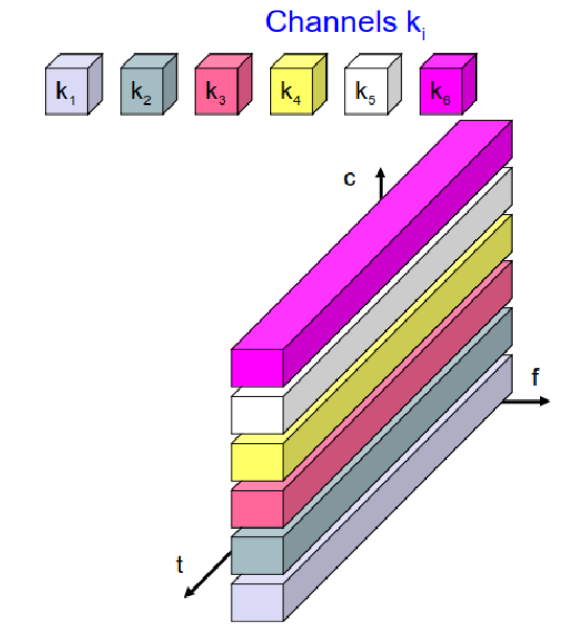
\includegraphics[width=0.4\textwidth]{img/wireless/CDMA.png}
        \caption{Example of CDMA}
        \label{fig:CDMA}
      \end{figure}
    \end{subsubsection}
    \begin{subsubsection}{TDM/A + FDM/A}
      It is also possible to combine the two methods.
      We can combine the time and frequency division multiplexing, allowing to divide the available
      bandwidth over multiple logical channels, by assigning a different time slot and frequency band
      to each user.\\
      With this solution, we are able to achieve a better degree of protection against tapping
      and frequency selective interference, at the cost of higher data rates(compared to CDMA).\\
      This method also requires a precise coordination between the users.\\
      \begin{figure}[h]
        \centering
        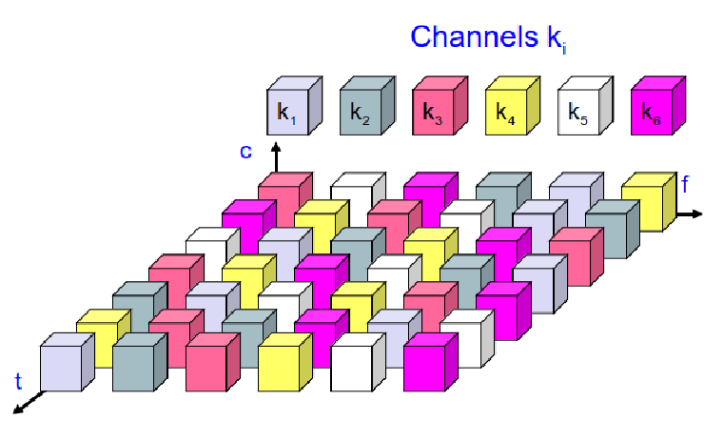
\includegraphics[width=0.4\textwidth]{img/wireless/TFDM.png}
        \caption{Example of TDMA/FDMA}
        \label{fig:TDMA/FDMA}
      \end{figure}
    \end{subsubsection}
  \end{subsection}

  \begin{section}{Source and channel coding}
    A brief overview: we have a source that generates a message, which is then encoded by the source
    encoder, to limit the amount of bits transmitted and the effects of noise.\\
    Those bits are then transformed into waveforms, which are altered by the channel, and then
    transformed back into bits by the channel decoder, after inverting the effects of the channel.\\

    Part of this operation are carried out in two steps:
    \begin{itemize}
      \item \textbf{Encoding}: which aims to produce a compressed representation $Y$ of the original
        message $X$. Usually encoding is simply a function $f$ that maps $X$ to $Y$.
      \item \textbf{Decoding}: which aims to recover the original message $X$ from the representation
        $Y$. Usually decoding is simply a function $f^{-1}$ that maps $Y$ to $X$.
    \end{itemize}
    \begin{figure}[h]
      \centering
      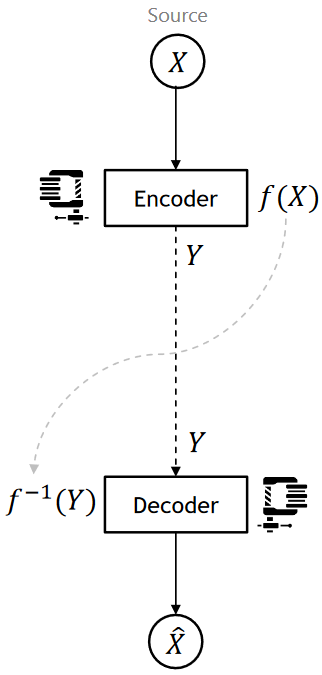
\includegraphics[width=0.2\textwidth]{img/wireless/encoding and decoding.png}
      \caption{General schema of encoding and decoding}
      \label{fig:encoding and decoding}
    \end{figure}

    \begin{subsection}{Source Coding}
      We would like to choose a encoding function $f$ that can be reverted while also \textbf{reducing
        redundancy} in the message.\\
        \begin{boxH}
          \textbf{Source coding}, also known as data compression, aims to represent information or
          data in a more compact form to reduce redundancy and save storage space or transmission 
          bandwidth.
        \end{boxH}
        This is possible because many real-world datasets exhibit patterns or repetitions that can 
        be efficiently encoded

        \begin{figure}[h]
          \centering
          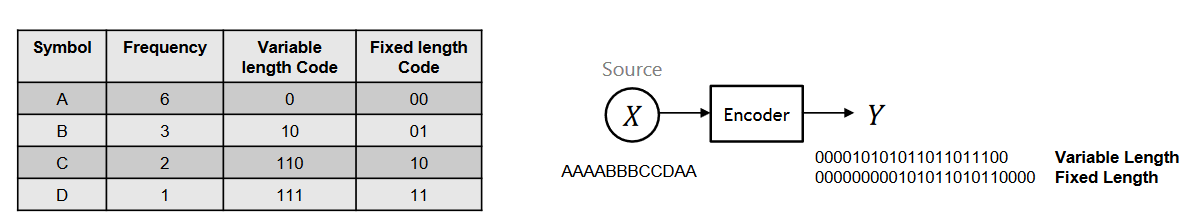
\includegraphics[width=\textwidth]{img/wireless/source coding.png}
          \caption{Example of source coding}
          \label{fig:source coding}
        \end{figure}

        Figure \ref{fig:source coding} shows an example of source coding. The example supposes that
        a sequence of letters is being transmitted. A possible uncompressed representation of the 
        letters would be assigning a two bit code to each letter(fixed length code).\\
        An alternative strategy exploits the fact that some letters are more frequent than others,
        assigning shorter codes to the most frequent letters(variable length code). With this
        solution, we are able to reduce the number of bits needed to transmit the message.\\
        \begin{subsubsection}{Compression Types}
          There are two main compression classes:
          \begin{itemize}
            \item \textbf{Lossless Compression}: the original data can be perfectly reconstructed
              from the compressed data($\hat{X}=X$). This is useful when the original data must be 
              preserved exactly, such as in text or executable files. Some examples of lossless
              compression includes ZIP, RAR, and PNG.
            \item \textbf{Lossy Compression}: the original data cannot be perfectly reconstructed
              from the compressed data($\hat{X}\approx X$). This is useful when the original data 
              can be approximated or when some loss of quality is acceptable, such as in images 
              or audio files.
          \end{itemize}
          As there are no officials compression formats, the specifications are defined by the
          fidelity requirements of the application. Generally, there is a trade-off between the
          compression efficiency and the computational complexity of the algorithm.
        \end{subsubsection}
    \end{subsection}

    \begin{subsection}{Error Detection and Correction}
      After compression, all the redundancy of the message has been possibly removed, and the bits
      that make up the message are the ones to be transmitted.\\
      Ideally, the message should be received unaltered, but we know that the channel can introduce
      errors in the message.\\
      Error detection techniques allow detecting such errors, while error correction enables 
      reconstruction of the original data. But those schemes add some redundancy to the message.\\
      For doing this, there are two main approaches:
      \begin{itemize}
        \item \textbf{Automatic Repeat request(ARQ)}: it implements acknowledgements and timeouts
          to ensure that the message is correctly received. 
        \item \textbf{Forward Error Correction(FEC)/Channel coding}: it adds redundancy to the 
          message to allow
          the receiver to correct errors without the need for retransmission.
      \end{itemize}
      \begin{subsubsection}{Channel Coding}
        Channel coding aims to detect and correct errors that may occur during transmission.\\
        It adds redundant bits to the original message, creating a coded message that contains 
        extra information for error detection and correction.\\
        The effectiveness of a channel code is often measured by its error correction capability,
        indicating the maximum number of errors that can be corrected within a codeword.\\

        There are two main types of channel coding:
        \begin{itemize}
          \item \textbf{Block Codes}: the message is divided into blocks of fixed length, and a 
            fixed number of redundant bits are added to each block. The receiver uses the redundant
            bits to detect and correct errors.
          \item \textbf{Convolutional Codes}: the message is encoded using a convolutional encoder,
            which adds redundant bits based on the current and previous bits of the message. The 
            receiver uses a Viterbi decoder to detect and correct errors.
        \end{itemize}
      \end{subsubsection}
      \begin{subsubsection}{Block Codes}
        A block code acts on block of $k$ bits of input data to produce $n$ bits of output data.
        This operation is carried out by the channel encoder.\\
        It simply adds $n-k$ bits of redundancy to the original message, which can be used by the
        receiver to detect and correct errors.\\

        \begin{figure}[h]
          \centering
          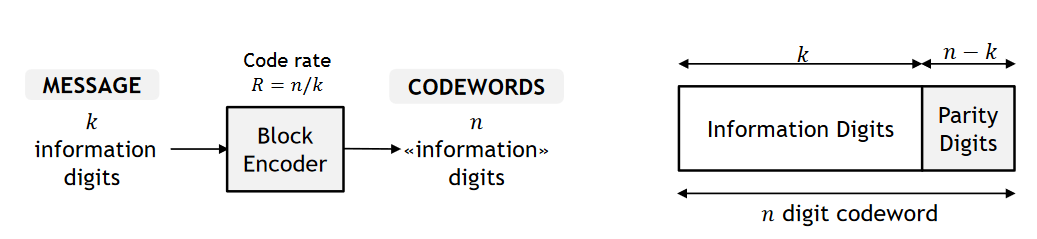
\includegraphics[width=\textwidth]{img/wireless/block codes.png}
          \caption{Example of block code}
          \label{fig:block code}
        \end{figure}
      \end{subsubsection}
    \end{subsection}
  \end{section}
  \begin{section}{Questions and answers}
    \begin{subsubsection}{In a digital communication system, what is the role of source encoding and
      decoding? What is its main goal? Describe the working principle(s)}
      In a digital communication system, the communication is, as the name suggests, digital. The
      thing is, the channel is only able to carry analog signals, meaning that we need an interface
      to convert the digital signal into a an analog one, and vice versa. The user portion of the
      interface section of a digital communication schema, at first apply source encoding, reducing
      the number of bits to be stransmitted, and channel encoding, which makes the sequence more
      robust, all this in a modulator, and the data is at last converted to analog by an encoder.
      The receiver gets the analog signals and sample it with a decoder, from which a demodulator is
      able to retreive the digital data, even perfectly if the sample frequence is high enough, by
      doing channel and source decoding, which corrects errors and recovers the original message.
    \end{subsubsection}

    \begin{subsubsection}{Describe how different signals can coexist over the same wireless medium.}
      Different signals can coexist over the same shared medium thanks to a method called
      multiplexing, which allows to divide the available bandwidth over multiple logical channels.
      There are different multiplexing schemes:
      \begin{itemize}
        \item Frequency division multiplexing: thanks to the modulation and demodulation of signals,
          we can transmitt different signals with overlapping bandwidth, by modulating each signal
          at a different frequency. This schema require a guard band between channels to avoid
          interference, and it is basically used by all wireless systems, because each channel has
          access to the full bandwidth for the whole time.
        \item Time division multiplexing: the bandwidth is divided between the logical channels 
          by assigning a time slot to each user, even if no data has to be transmitted.
        \item Code division multiplexing allows to divide the available bandwidth over multiple
          logical channels, by assigning a different code to each user, which is used to separate
          the signal from the others, which share the same spectrum at the same time, by exploiting
          the orthogonality between signals.
      \end{itemize}
    \end{subsubsection}

    \begin{subsubsection}{Describe the tradeoff between bandwidth efficiency and energy efficiency
      in digital modulations.}
      We know that to achieve a higher bandwidth efficiency, one has to use a lower bandwidth. 
      Symbols are distributed over the bandwidth, and the larger the energy, the larger
      the bandwidth, and thus the distance between symbols. With a smaller bandwidth, those are
      cramped in a smaller "space". But using a smaller bandwidth means that we are using a larger
      base pulse, which occupies less bandwidth but require more energy. This means that if we
      choose to occupy a smaller bandwidth, the transmitted sequence is more prone to errors,
      because symbols are closer to each other, and require less energy to be transmitted. on the
      other hand, if we add more space inbetween symbols, we will occupy a larger bandwidth, which
      requires less energy to be transmitted and is less prine to errors.
    \end{subsubsection}

  \end{section}
\end{section}

\chapter{Security at the physical layer}
As already mentioned in section \ref{sec:intro}, the wireless channel has no inherent security mechanisms. 
As a result, The wireless communication medium is open to \textbf{jamming} (or interference) and 
\textbf{eavesdropping} attacks from intruders.\\
Furthermore, the attacks can be classified into two categories: 
\begin{itemize}
    \item \textbf{Passive attacks}: the attacker only listens to the communication between the 
      two parties, without disrupting the network operation.
    \item \textbf{Active attacks}: the attacker can interfere in the communication between the 
      two parties.
\end{itemize}
\begin{figure}[H]
    \centering
    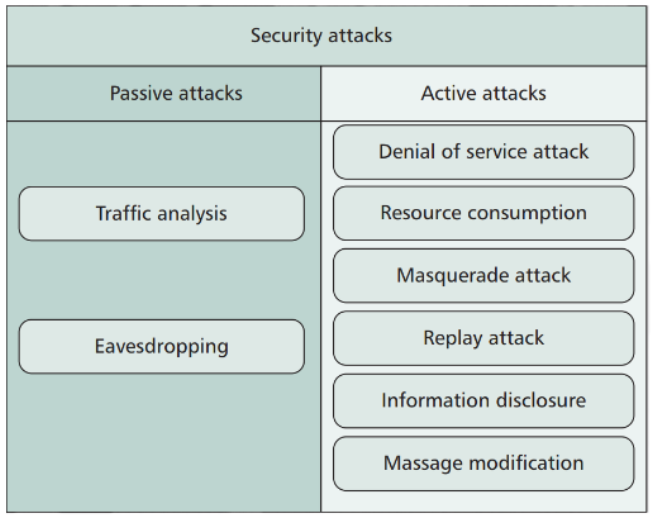
\includegraphics[width=0.5\textwidth]{img/wireless/attack classification.png}
    \caption{Active and passive attacks}
    \label{fig:active_passive_attacks}
\end{figure}
We are going to go through some of the most common attacks in wireless communication.
\begin{section}{Jamming}
   \begin{boxH}
     Jamming is a simple strategy to disrupt wireless communication by interfering with the
     communication channel.
    \end{boxH}
    It is usually carried out by broadcasting an interfering signal on a broad spectrum of frequencies
    to block the communication.\\
    A persistent and powerful adversary can always jam all data transmissions by transmitting 
    high-power white noise over the entire frequency spectrum.
    Jammer can be classified into two categories:
    \begin{itemize}
      \item \textbf{Active jamming}: the attacker continuously transmits a jamming signal to 
        interfere with the communication.
      \item \textbf{Reactive jamming}: the attacker only transmits a jamming signal when it
        detects a signal from the legitimate transmitter.
    \end{itemize}
    Although jamming is a difficult to address availability issue, it can be addressed via many
    physical layer security techniques.
    \end{section}
    \begin{section}{Eavesdropping}
      The wireless communication channel is a broadcast medium by nature. Because of this its 
      hard to eliminate unauthorized access to the wireless channel.\\
      To address those problesm, the most common way is to encrypt the data before transmitting it.\\
      Another widely used approach is to force the transmitter and receiver to adopt some 
      information hiding measures, by embedding private messages into a background signal or 
      noise process. In other words, we bury the information in the noise.\\
      Eavesdropping too can be addressed via physical layer security techniques.
\end{section}

\begin{section}{Physical Layer Security}
  In traditional systems, reliability is guaranteed by channel coding at the physical layer, while 
  security is ensured by encryption protocols at the upper layers, although in some cases we would 
  like to have security at the physical layer.\\
  This is possible because the physical layer has some unique properties that can be exploited to
  provide security, nominally the randomness of the wireless channel, which is an unpredictable
  and time-varying medium.\\

  \begin{boxH}
    \textbf{Physical layer security} aims at \textbf{exploiting the randomness} inherent in noisy channels to provide
    an additional level of protection at the physical layer.
  \end{boxH}
  
  \begin{figure}[h]
    \centering
    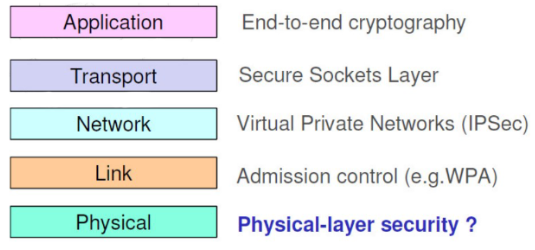
\includegraphics[width=0.5\textwidth]{img/wireless/layer security.png}
    \caption{Security measures at different layers}
    \label{fig:layer_security}
  \end{figure}
  A desirable proprety of the communication channel is \textbf{perfect secrecy}, which for a 
  wireless communication channel means that the channel is unknown to unauthorized users, or the 
  channel of the unauthorized users is more noisy than that of the authorized users.\\
  This means that we have a "better" channel than the eavesdropper, and we can obtain a that in 
  a different ways. For instance the sender and the receiver can cooperate, for example by choosing
  the same channel estimation method.\\

  In any case, security at physical layer is not intended to replace cryptographic security, but rather, it
  affords an additional protection layer. In fact, Physical Layer Security does not even allow 
  demodulation, which cryptographic security does.\\
  Nowadays, many results from information theory, signal processing, and cryptography
  suggest that there is much security to be gained by accounting for the imperfections of the
  physical layer when designing secure systems.

  Furthermore, physical layer security methods can be categorized into:
  \begin{itemize}
    \item \textbf{channel approaches}: such as fingerprinting, precoding and applying MIMO techniques.
    \item \textbf{code approaches}: adding cryptografy to error correction codes and applying spreading
      codes to the signal.
    \item \textbf{power approaches}: using direction antennas to make the communication less broad 
      or generating artificial noise to confuse the eavesdropper.
    \item \textbf{signal design approaches}: using artificial noise to degrade eavesdropper's 
      channel estimation
  \end{itemize}

  Each method addresses specific aspects of physical layer security, ranging from utilizing
  channel characteristics to employing artificial noise and directional antennas, and each one 
  is effective against different types of attacks.
  \begin{figure}[H]
    \centering
    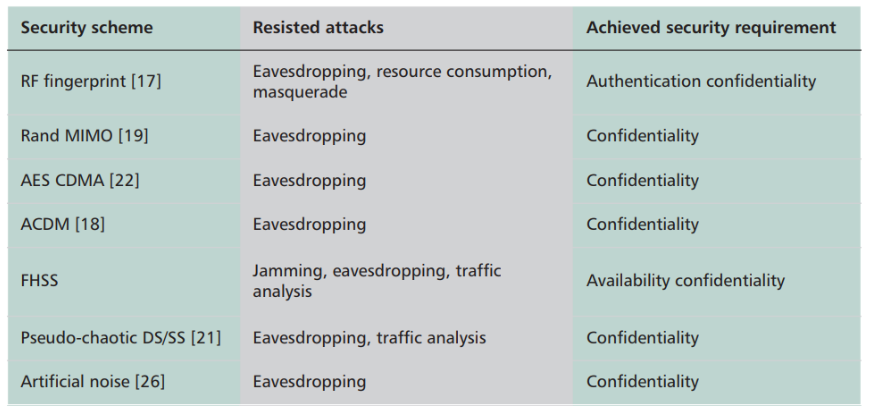
\includegraphics[width=0.8\textwidth]{img/wireless/physical layer security schema.png}
    \caption{Physical layer security methods}
    \label{fig:physical_layer_security_schema}
  \end{figure}

\end{section}


\chapter{GNSS and positioning}
  Global Navigation Satellite Systems (GNSS) are satellite-based systems that provide positioning, 
  navigation, and timing (PNT) services to users worldwide. The most well-known GNSS is the Global 
  Positioning System (GPS).\\
  The use of GPS and other GNSSs has become quite common in several civil application fields, (e.g.,
  transports and personal mobility, agriculture, ICT, ...), so Location Based Services (LBS) are
  becoming more and more important.\\

  In this chapter we will that GNSS users are particularly sensitive to some kinds of attacks, because
  those signals are very weak: for example Replaying broadcast GNSS signals with some delay 
  (meaconing), is enough to trick a user into a wrong position.\\
  \begin{section}{The positioning Problem}
    First of all, we need to define what is a position.\\
    \begin{boxH}
      A position is a set of coordinates, one for each dimension, associated with a reference 
      system.
    \end{boxH}
    \begin{figure}[h]
      \centering
      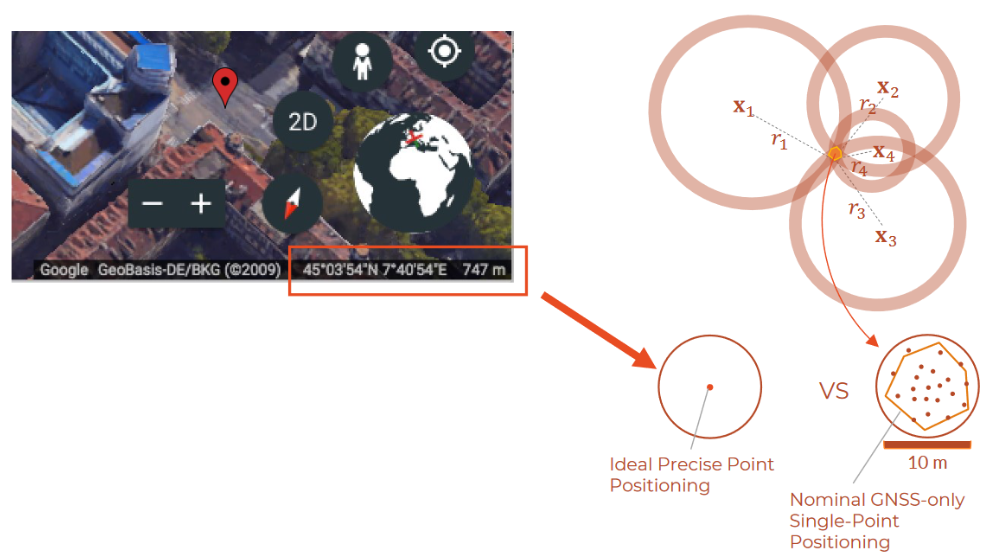
\includegraphics[width=0.8\textwidth]{img/wireless/GNSS position.png}
      \caption{Positioning in a 3D space}
      \label{fig:GNSS position}
    \end{figure}
    As shown in picture \ref{fig:GNSS position}, ideally we would like to have a system that can
    get a precise point positioning over a space, but in reality what we get is a cloud of points
    around the real position, from which the real position is estimated, withing a certain confidence
    interval.\\

    That being said, how is a position estimated?\\
    The information needed to estimate a position is provided by a set of sensors installed on 
    a terminal, such as a smartphone or a GPS receiver.\\
    Some of the most common sensors used are:
    \begin{itemize}
      \item \textbf{Satellite Navigation Chipset}, such as a GPS sensor, which tracks the signals
        from the satellites.
      \item \textbf{Inertial systems}, such as accelerometers and gyroscopes that measure the 
        acceleration and the angular velocity of the terminal.
      \item \textbf{Electronic Compasses}, which provide the orientation of the terminal.
      \item \textbf{Barometers}, which measure the atmospheric pressure.
      \item $\dots$
    \end{itemize}

    Because using all that sensors together to estimate a position is ideal but quite complex,
    a \textbf{data fusion algorithm} is used to combine the information from the sensors and estimate
    the position.\\
    \begin{figure}[h]
      \centering
      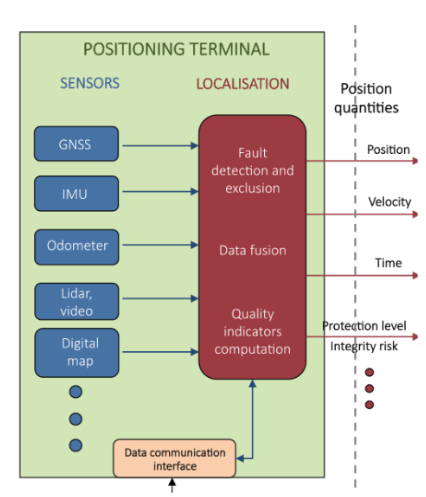
\includegraphics[width=0.3\textwidth]{img/wireless/data fusion algorithms.png}
      \caption{Representation of a data fusion algorithm}
      \label{fig:GNSS data fusion}
    \end{figure}
    In some cases using only the information provides is not enough to estimate a position, so
    some \textit{tricks} are used to improve the accuracy of the position estimation.\\
    For example google maps, when it gets an off road position, uses the information provided and
    maps the position to a point between some landmarks positioned on the road, as shown in picture
    \ref{fig:maps example}.\\

    \begin{figure}[h]
      \centering
      \includegraphics[width=0.6\textwidth]{img/wireless/maps example.png}
      \caption{Example of position estimation using landmarks}
      \label{fig:maps example}
    \end{figure}
  \end{section}

  \begin{section}{Satellite Navigation Systems and Segments}
    A little of history: the first satellite navigation system was put in space by the US Department
    of Defense in 1978. But it was only in the early 2000s that the system was opened to civil users.\\
    The european counterpart of the GPS is the Galileo system, which was put in space in 2017.\\
    \begin{figure}[h]
      \centering
      \includegraphics[width=0.9\textwidth]{img/wireless/GNSS history.png}
      \caption{History of GNSS systems}
      \label{fig:GNSS systems history}
    \end{figure}
    To provide a global coverage, a GNSS system is composed of a constellation of satellites, which
    are positioned in such a way that at least 4 satellites are visible from any point on the Earth.\\

    There are 4 main GNSS systems nowadays:
    \begin{itemize}
      \item \textbf{GPS} (USA)
      \item \textbf{Galileo} (Europe)
      \item \textbf{GLONASS} (Russia)
      \item \textbf{Beidou} (China)
    \end{itemize}
    which orbits at different altitudes and inclinations.\\
    Each of those systems  continuously transmit navigation signals in different frequencies in $L$ 
    band, as shown in picture \ref{fig:GNSS band}.\\

    \begin{figure}[h]
      \centering
      \includegraphics[width=0.8\textwidth]{img/wireless/GNSS band.png}
      \caption{Division of the $L$ band for GNSS systems}
      \label{fig:GNSS band}
    \end{figure}

    All those system are composed of 3 main segments:
    \begin{itemize}
      \item \textbf{Space Segment}, which is composed of the satellites, which continuously transmit
        the signals.
      \item \textbf{Control Segment}, which is composed of the ground stations that monitor the 
        satellites and send them the corrections.
      \item \textbf{User Segment}, which is composed of the users that receive the signals from the
        satellites and estimate their position. It performs 3 core functions:
        \subitem - Identification of the satellites in view
        \subitem - Measurement of the user-satellite distance
        \subitem - Run a PVT(Position, Velocity, Time) estimation algorithm
    \end{itemize}
    \begin{figure}[h]
      \centering
      \includegraphics[width=0.2\textwidth]{img/wireless/GNSS segments.png}
      \caption{Schema of the GNSS segments}
      \label{fig:GNSS segments}
    \end{figure}
    \begin{subsection}{GNSS signals}
      The GNSS satellites continuously transmit navigation signals in different frequencies in $L$ 
      band.\\
      Those signals are made up of different components, as shown in picture \ref{fig:GNSS signals}.\\
      The carrier modulate the data at the right frequency, the spreading code to perform multiple
      access, allowing to distinguish information from different satellites and demultiplexing the
      signals from the same satellite, , and the navigation data that contains the information 
      about the satellite position and the time.\\

      The navigation data allow the user to compute the travelling time from the satellite to the receiver,
      and the satellite position at any time.\\
      Using both the satellite position and the travelling time, the user can estimate its position
      , velocity and time(PVT).\\

      \begin{figure}[h]
        \centering
        \includegraphics[width=0.8\textwidth]{img/wireless/GNSS signal scheme.png}
        \caption{Scheme of the signals that make up the GNSS signal}
        \label{fig:GNSS signals}
      \end{figure}
    \end{subsection}

  \end{section}
  \begin{section}{Multilateration}
    Lets take a look at figure \ref{fig:GNSS multilateration problem}.\\
    We have a satellite that sends a signal $R_i$ to a user $x$, which would like to estimate 
    three coordinates $\langle x, y, z \rangle$.\\
    The signal contains the position of the satellite and the departure time of the message
    $T_{TX}$.\\
    The receiver measures the arrival time of the signal $T_{RX}$, and computes the distance
    between the receiver and the satellite $R_i$ as follows:
    \begin{equation}
      R_i = c\cdot \tau = c(T_{RX} - T_{TX})
      \label{eq:GNSS distance}
    \end{equation}
    where $c$ is the speed of light, which is the propagation speed of the signal, and $\tau$ is the
    \textit{time of flight} of the signal.\\
    In other words, the distance is the traveling time of the signal multiplied by propagation time
    in the free space.\\

    \begin{figure}[h]
      \centering
      \includegraphics[width=0.8\textwidth]{img/wireless/GNSS multilateration problem.png}
      \caption{Multilateration problem}
      \label{fig:GNSS multilateration problem}
    \end{figure}

    One measurement is not enough to estimate the position of the receiver, so at least 3 measurements
    are needed.\\
    \begin{boxH}
      We call this procedure \textbf{multilateration}, or the process of determining the position of an object
      by measuring the time of arrival of the signals from multiple sources.
    \end{boxH}

    But knowing the distance only tells us that the receiver is on a sphere centered on the satellite
    with radius $R_i$. It can be at any point on the sphere.\\
    If we have 2 satellites, we have 2 spheres, and the receiver is at the intersection of the two
    spheres.\\
    If we have 3 satellites, we have 3 spheres, and the receiver is at the intersection of the 3
    spheres.\\
    Unfortunately things are never that simple, but it gives the rough idea of how multilateration
    works.\\

    \begin{figure}[h]
      \centering
      \includegraphics[width=\textwidth]{img/wireless/multilateration comparison.png}
      \caption{Multilateration with 1, 2 and 3 satellites}
      \label{fig:Multilateration comparison}
    \end{figure}
  \end{section}
  \begin{section}{GNSS Functional basics}
    Lets add more detail to multilateration.\\
    If a satellite trasmit a pulse at time $t_0$, the receiver will receive it at time $t_0+\tau$,
    where $\tau$ is the time it takes for the signal to travel from the satellite to the receiver.\\
    We already saw in equation \ref{eq:GNSS distance} that the distance between the satellite and the
    receiver is equal to the time of flight of the signal multiplied by the speed of light.\\

    To get the distance, we only need to timestamp correctly the time of arrival of the signal.
    Yet, calculating the time of flight is not that simple, because the satellite and the receiver
    must be \textbf{synchronized} to allow the transmission time and the reception time to be on the 
    same time scale, and to be precise. Otherwise the distance estimation would be very off: 
    a signal that travels at the speed of light for 1 second travels 300000 km.\\
    In fact, the satellite host an \textbf{atomic clock}, which is a very precise clock that allows
    the satellite to timestamp the signal with a very high precision. They are also synchronized thanks
    to the control segment.\\
    The receiver also has a clock, but it is most likely not as precise as the atomic clock. 
    For this reason, the bias of the user torward the GNSS time scale $\delta t_u$ is unknown.\\
    The measured distance is then different from the geometric range and it is referred
    to as \textbf{pseudorange}, which is defined as:
    \begin{equation}
      \rho = c \cdot \tau + c \cdot \delta t_u
      \label{eq:GNSS pseudorange}
    \end{equation}

    There's also the bias of the satellite toward the scale $\delta t_u$. 
    This value is usually small and stable over time. The ground segment computes a bias $\delta t^S$
    that is uploaded to the satellite, and that the receiver can use to compute the right time of 
    flight.\\
    For those reason, we consider it to be zero, because it can be corrected.\\

    On the other hand, $\delta t_u$ cannot, the only thing we can do is keep it, so the position 
    is estimated by measuring the different pseudoranges from 4 different satellites, the minimum
    number of satellites in Line of Sight to estimate the position.\\
    This is because 3 satellites are needed to estimate the coordinates of a position, and the fourth
    satellite is needed to estimate the bias $\delta t_u$.\\
    If a larger number of satellites is in view a better estimation is possible.\\

    \begin{figure}[h]
      \centering
      \includegraphics[width=0.8\textwidth]{img/wireless/GNSS bias.png}
      \caption{Graphical representation of the bias $\delta t_u$ on the GNSS timescale}
      \label{fig:GNSS pseudorange}
    \end{figure}

    To sum it up, in GNSSs the user position is obtained through:
    \begin{itemize}
      \item \textbf{satellites} that broadcast that transmits timestamps.
      \item \textbf{Pseudoranges}, estimated trough one-way-arrival measurements
        receiver, plus the bias of the user toward the GNSS time scale.
      \item \textbf{Multilateration} based on the measurements
    \end{itemize}

    \begin{subsection}{The estimation problem}
      We have the measurements, but we need to estimate the position of the receiver.\\
      The relationship between the pseudoranges can be written as:
      \begin{equation}
        \begin{cases}
          \rho_1 = \sqrt{(x_1 - x_u)^2 + (y_1 - y_u)^2 + (z_1 - z_u)^2} + c\delta t_u\\
          \rho_2 = \sqrt{(x_2 - x_u)^2 + (y_2 - y_u)^2 + (z_2 - z_u)^2} + c\delta t_u\\
          \rho_3 = \sqrt{(x_3 - x_u)^2 + (y_3 - y_u)^2 + (z_3 - z_u)^2} + c\delta t_u\\
          \rho_4 = \sqrt{(x_4 - x_u)^2 + (y_4 - y_u)^2 + (z_4 - z_u)^2} + c\delta t_u\\
        \end{cases}
        \label{eq:GNSS pseudorange relationship}
      \end{equation}
      where $\langle x_i, y_i, z_i \rangle$ are the coordinates of the satellites(which are known),
      and $\langle x_u, y_u, z_u \rangle$ are the coordinates of the user(which are unknown as the bias).

      The goal is to invert the relationship and find the user coordinates and the bias given the
      pseudoranges.\\
      It is a non-linear estimation problem which is linearized through Taylor expansion 
      And solved through Least Mean Square Solutions or Bayesian Filters (e.g. Kalman).\\

      The generic pseudorange, which is a nonlinear relationship,
      \begin{equation*}
        \rho_i = \sqrt{(x_i - x_u)^2 + (y_i - y_u)^2 + (z_i - z_u)^2} + c\delta t_u
      \end{equation*}
      can be approximated through the Taylor expansion around a known location used as a linearization point
      (a point that is close to the real solution) $\langle \hat{x}_u, \hat{y}_u, \hat{z}_u, \hat{\delta t}_u \rangle$:
      \begin{equation*}
        \hat{\rho}_i = \sqrt{(x_i - \hat{x}_u)^2 + (y_i - \hat{y}_u)^2 + (z_i - \hat{z}_u)^2} + c\hat{\delta t}_u
        \label{eq:GNSS linearization}
      \end{equation*}
      To put it into a graphical prospective, take a look at figure \ref{fig:GNSS linearization}.\\
      If we choose a linearization point, we need to know the difference $\Delta x_u$ between the real
      position and the linearization point. If we can estimate it, which is easier because it is a 
      linear problem, we can estimate the user position.\\


      \begin{figure}[h]
        \centering
        \includegraphics[width=0.5\textwidth]{img/wireless/linearization scenario.png}
        \caption{Graphical representation of the linearization of the pseudorange in one dimension}
        \label{fig:GNSS linearization}
      \end{figure}
      We can expand this concept to the general formula \ref{eq:GNSS linearization} as the difference 
      between the real position and the linearization point:
      \begin{equation}
        \begin{cases}
          \Delta x_u = x_u - \hat{x}_u\\
          \Delta y_u = y_u - \hat{y}_u\\
          \Delta z_u = z_u - \hat{z}_u\\
          \Delta \delta t_u = \delta t_u - \hat{\delta t}_u\\
        \end{cases}
        \label{eq:GNSS linearization difference}
      \end{equation}
      The linearized pseudorange can be written as:
      \begin{equation}
        \delta \rho_j = \hat{\rho}_j - \rho_j = a_{xj}\Delta x_u + a_{yj}\Delta y_u + a_{zj}\Delta z_u + a_{tj}\Delta \delta t_u
        \label{eq:GNSS linearized pseudorange}
      \end{equation}
      The coefficients $a_{ij}$ are the partial derivatives of the pseudorange with respect to the
      user position and the bias, obtained through the Taylor expansion.\\
      They can be written as:
      \begin{equation}
        \begin{cases}
          a_{xj} = \dfrac{x_j - \hat{x}_u}{\hat{\rho}_j}\\
          a_{yj} = \dfrac{y_j - \hat{y}_u}{\hat{\rho}_j}\\
          a_{zj} = \dfrac{z_j - \hat{z}_u}{\hat{\rho}_j}\\
          a_{tj} = \dfrac{c}{\hat{\rho}_j}
        \end{cases}
        \label{eq:GNSS linearized coefficients}
      \end{equation}
      where 
      \begin{equation*}
        \hat{\rho}_j = \sqrt{(x_j - \hat{x}_u)^2 + (y_j - \hat{y}_u)^2 + (z_j - \hat{z}_u)^2} + c\hat{\delta t}_u
      \end{equation*}
      that being the geometrical distance between the linearization point and the satellite.\\
      This allows us to write our relationship as:
      \begin{equation}
        \begin{cases}
          \delta \rho_1 = a_{x1}\Delta x_u + a_{y1}\Delta y_u + a_{z1}\Delta z_u + a_{t1}\Delta \delta t_u\\
          \delta \rho_2 = a_{x2}\Delta x_u + a_{y2}\Delta y_u + a_{z2}\Delta z_u + a_{t2}\Delta \delta t_u\\
          \delta \rho_3 = a_{x3}\Delta x_u + a_{y3}\Delta y_u + a_{z3}\Delta z_u + a_{t3}\Delta \delta t_u\\
          \delta \rho_4 = a_{x4}\Delta x_u + a_{y4}\Delta y_u + a_{z4}\Delta z_u + a_{t4}\Delta \delta t_u\\
        \end{cases}
        \end{equation}
        that can be also rewrited in a matrix form as:
        \begin{equation}
        \begin{bmatrix}
          \delta \rho_1\\
          \delta \rho_2\\
          \delta \rho_3\\
          \delta \rho_4\\
        \end{bmatrix}
        =
        \begin{bmatrix}
          a_{x1} & a_{y1} & a_{z1} & a_{t1}\\
          a_{x2} & a_{y2} & a_{z2} & a_{t2}\\
          a_{x3} & a_{y3} & a_{z3} & a_{t3}\\
          a_{x4} & a_{y4} & a_{z4} & a_{t4}\\
        \end{bmatrix}
        \begin{bmatrix}
          \Delta x_u\\
          \Delta y_u\\
          \Delta z_u\\
          \Delta \delta t_u\\
        \end{bmatrix}
        \label{eq:GNSS linearized matrix}
      \end{equation}
      where $a_{tj}$ can be approximated as $1$ because the bias is usually small.\\
      This matrix representation is easier to invert, in fact 
      \begin{equation*}
        \delta x= H^{-1}\delta \rho
      \end{equation*}
      which is our solution: the user position.\\
      \begin{subsubsection}{The Least Squares Solution}
        The method above can only be used if the number of satellites is small(4 or less), because 
        otherwise the matrix $H$ would be non-square and non-invertible.\\
        If the number of satellites is larger, it is possible to use the Least Squares Solution.\\
        The solution would be 
        \begin{equation}
          \Delta x = (H^TH)^{-1}H^T\delta \rho
          \label{eq:GNSS least squares}
        \end{equation}
        where $H^T$ is the transpose of the matrix $H$.\\
      \end{subsubsection}
      \end{subsection}

    \begin{section}{Positioning Errors}
      We know that that channel is unpredictable, so the pseudorange is most likely affected by errors,
      due to things such as noise and propagation.\\
      We can redifine our pseudorange model as:
      \begin{equation}
        \rho_i = \sqrt{(x_i - x_u)^2 + (y_i - y_u)^2 + (z_i - z_u)^2} + b_{ut} + \epsilon
        \label{eq:GNSS pseudorange error}
      \end{equation}
      where $b_{ut}$ is the bias of the user toward the GNSS time scale, and $\epsilon$ is the error.\\

      We also need to modify the solution accordingly:
      \begin{equation}
        \Delta x = [(H^TH)^{-1}H^T]\delta \rho
        \label{eq:GNSS least squares error}
      \end{equation}
      where $\delta \rho$ is the error in the pseudoranges.\\
      Basically, we have a portion of the formula that depends on the geometry of the satellites(
      $(H^TH)^{-1}H^T$) and a portion that depends on the errors in the pseudoranges which is
      upredictable.\\
      As it is possible to observe, the position of the satellite influence the error in the pseudorange,
      fore example amplifying it.\\
      
      The causes of the errors in the pseudorange are shown in figure \ref{fig:GNSS errors}.\\
      The relativistic effect on the clock, the fact that even if the clocks are synchronized, they
      move at different speeds, can be corrected because it is predictable.\\
      The atmoshpere too influences the signal, but it can be corrected because it is predictable.\\
      Some of them cannot be corrected, such as the multipath effect, the fact that the signal can
      bounce off buildings and arrive at the receiver later than expected.\\

      \begin{figure}[h]
        \centering
        \includegraphics[width=0.8\textwidth]{img/wireless/GNSS errors.png}
        \caption{Causes of the errors in the pseudorange}
        \label{fig:GNSS errors}
      \end{figure}

      \begin{subsection}{User Equivalent Range Error}
        The summary of the total error budget affecting a pseudorange from the user's point of view 
        is called the \textbf{user equivalent range error} (UERE).\\
        Thus, we can model the pseudorange error as a random variable with a mean of $0$ and a standard
        deviation of $\sigma_{\text{UERE}}$.\\
        After correcting known sistematic errors, the unknown ones can be modelled as a Gaussian 
        distribution, with a mean of $0$ and a variance $\sigma_{\text{UERE}}^2$, obtained as the sum
        of other residual contributions:
        \begin{equation}
          \sigma_{\text{UERE}} = \sqrt{\sum_{j} \sigma^2_j [m]}
        \label{eq:GNSS UERE}
      \end{equation}
      \end{subsection}

      \begin{subsection}{The Geometrical Factor}
        Errors makes the solution more uncertain, but its not the only factor that influences the
        accuracy of the solution.\\
        The geometrical distribution of satellites affects the precision of estimated position too

        \begin{figure}[h]
          \centering
          \includegraphics[width=0.7\textwidth]{img/wireless/satellite distibution.png}
          \caption{Distrubution of the satellites ideally and in reality}
          \label{fig:GNSS geometry}
        \end{figure}

        It can be proved that, under some conditions, this geometrical effect on the positioning 
        error can be measured.
        the standard deviation of the positioning error can be obtained as:
        \begin{equation}
          \sigma_{x} = \sqrt{\sigma^2_{x_u} + \sigma^2_{y_u} + \sigma^2_{z_u} + \sigma^2_{b_{ut}}}
          =\text{GDOP} \cdot \sigma_{\text{UERE}}
          \label{eq:GNSS PDOP}
        \end{equation}
        where GDOP is the \textbf{Geometric Dilution of Precision}:
        \begin{equation}
          \text{GDOP} = \sqrt{tr\{[H^TH]^{-1}\}}
          \label{eq:GNSS GDOP}
        \end{equation}
        and $\sigma_{\text{UERE}}$ is the standard deviation of the pseudorange error.\\
      \end{subsection}
    \end{section}

    \end{section}

    \begin{section}{GNSS threats}
      GNSS is not that robust by itself, in fact the main source of signal degradation are:
      \begin{itemize}
        \item \textbf{evil waveforms}
        \item \textbf{multipath}
        \item \textbf{radio frequency interference}
        \item \textbf{spoofing}
      \end{itemize}
      The robustness of GNSS signals derives from the \textbf{spread spectrum} nature of the 
      transmitted signal (Direct Sequence Spread Spectrum), exploited also for CDMA purposes.\\
      Despite the spread signal structure, navigation receivers are vulnerable to (strong) 
      interfering signals, that might prevent the correct signal processing.\\

      In fact, the typical signal to noise ration of a GNSS signal is around $-30dB$, which 
      means that on normal conditions the signal is buried in the noise.\\
      Fortunately, spread spectrum is robust to the presence of interfering signals, but we still
      have to revert the spreading to recover the original signal.\\
      The product with the PRN code spreads the power over a larger bandwidth, making the bandwidth
      of a signal $B_x \simeq 50 - 250\text{Hz}$ much larger($B_{SS} \simeq 2-8\text{MHz}$).\\
      If an interference signal of bandwidth $B_i$ affects the signal, only a portion of the power 
      will be actually received as “additional noise”, because the rest of the power will be
      spread over the whole bandwidth.\\

      For this reason, the despreading operation made at the receiver spreads the power of the 
      interfering signal over a wide bandwidth($B_{SS}$), making the interference power density
      much lower than the signal power density.\\

      \begin{figure}[h]
        \centering
        \includegraphics[width=0.9\textwidth]{img/wireless/signal despreading.png}
        \caption{Effect of despreading over a signal bandwidth}
        \label{fig:GNSS despreading}
      \end{figure}
      \begin{subsection}{Interference classification}
        Because of the bandwidth size, we are actually able to classify interference, according to 
        the spectral and time features with relation to the GNSS signal:
        \begin{itemize}
          \item \textbf{Narrowband Interference}: $B_i \ll B_{SS}$
          \item \textbf{Wideband Interference}: $B_i \simeq B_{SS}$
          \item \textbf{Continuous Wave Interference}: the interference is continuous in time
            over a single frequency band, $B_i \to 0$
          \item \textbf{Pulse Interference}: the interference is pulsed in time
        \end{itemize}

        We can also distinguish between \textbf{Out-of-band interference} and \textbf{In-band
        interference}.\\
        The first one is interference that is outside the GNSS band, while the second one is
        interference that is inside the GNSS band. This means that OOB interference should not 
        affect the GNSS signal, while IB interference can, buth both of them can be problematic.\\

        \begin{figure}[h]
          \centering
          \includegraphics[width=0.7\textwidth]{img/wireless/in and out of band interference.png}
          \caption{Classification of interference}
          \label{fig:GNSS interference classification}
        \end{figure}

        A further distinction can be made between \textbf{Intentional Interference} and
        \textbf{Unintentional Interference}.\\
        The first one is interference that is intentionally generated to disrupt the GNSS signal,
        while the second one is interference that is generated by other devices, but that can still
        disrupt the GNSS signal, and is generally generated by OOB interference.\\
      \end{subsection}

      \begin{subsection}{Jamming}
        \begin{boxH}
          A \textbf{jammer} is a \textbf{device} that generates \textbf{interference} to disrupt the GNSS signal.\\
          Jamming objective is the denial of navigation service by masking the GNSS signal with
          noise.
        \end{boxH}

        Normally, signal radiation in the GNSSs bands is regulated by the ITU, and not legal.\\
        Those devices can be a severe threat for  liability-critical mass-market applications, 
        such as GNSS-based road tolling or fleet management.\\
        In general, Mass-market jammers usually aim at disturbing a wide band by 
        frequency-modulating a pure tone.\\

        Lets now try to understand the effect of jamming on the GNSS signal.\\
        In general, interference affect the receiver at different levels: at first we can observe 
        a spike in the noise level after the signal has been received, or we can observe a
        degradation of the signal quality.\\
        This means that we are able to understand if a signal is being jammed before the pseudorange
        is computed.\\

        The net effect is an error on the measured pseudorange $\rho$, and the effect depends on
        \begin{itemize}
          \item the receiver architecture(front-end filters, quantization bits, etc.)
          \item the structure of the GNSS signal(modulation, spreading, etc.)
        \end{itemize}
        Therefore detection and mitigation of interference can act at different stages of the 
        receiver itself:
        \begin{itemize}
          \item antenna shaping
          \item front-end filtering
          \item time domain blanking
          \item other transformed domains
        \end{itemize}

        \begin{figure}[h]
          \centering
          \includegraphics[width=0.7\textwidth]{img/wireless/jamming delay effect.png}
          \caption{Effect of jamming on the delay of a GNSS signal. The delay is increased by the
            jamming signal.}
          \label{fig:GNSS jamming effect}
        \end{figure}
        \begin{subsubsection}{Signal-to-Noise Ratio Monitoring}
          Aside from the spectrum, one other thing that can be monitored to detect jamming is the
          Signal-to-Noise Ratio(SNR).\\
          Strictly speaking, the interference is not noise, but from the user point of view it is
          indistinguishable from it. The net effect is that the SNR is affected by interference,
          contributing to the \textbf{noise variance}.\\

          Observing the SNR in some scenarios may allow to define a \textbf{statistical threshold}: 
          if the SNR is below a certain value, the signal may be jammed.\\

          Generally speaking, The only available output common to any GNSS receiver is the 
          carrier-to-noise-density ratio (C/N0) parameter, which is the ratio of the carrier power
          to the noise power spectral density, an estimated value closely related to SNR.\\
          The C/N0 is a good indicator of the signal quality, and it is used to detect jamming: in
          case of jamming, the C/N0 will decrease.\\
          \begin{figure}[h]
            \centering
            \includegraphics[width=0.3\textwidth]{img/wireless/c over n0.png}
            \caption{Example of a C/N0 measurements of a signal while being jammed.}
            \label{fig:GNSS CN0 monitoring}
          \end{figure}

        \end{subsubsection}
        \begin{subsubsection}{Spectral analysis}
          One of the most effective ways of detecting jamming is to perform a spectral analysis of the
          received signal.\\

          Figure \ref{fig:GNSS spectral analysis} shows the effect of interference on the spectrum
          of a GNSS signal.\\
          On the left is shown the effect of normal noise over the spectrum of the signal, while on
          the right is shown the effect of jamming.\\
          Is is evident when it is happening: you can clearly see it in the spectrum.\\

          \begin{figure}[h]
            \centering
            \includegraphics[width=0.7\textwidth]{img/wireless/spectrum effect.png}
            \caption{Effect of interference on the spectrum of a GNSS signal}
            \label{fig:GNSS spectral analysis}
          \end{figure}
        \end{subsubsection}
        \begin{subsubsection}{Automatic Gain Control Behavior}
          Another important detection strategy is to monitor the behavior of the Automatic Gain Control
          (AGC) of the receiver.\\

          The AGC is a system that automatically controls the gain of the receiver, in order to
          maintain the signal at a constant level, the optimal input range of the ADC(quantizer).\\
          \begin{figure}[h]
            \centering
            \includegraphics[width=0.4\textwidth]{img/wireless/AGC.png}
            \caption{Graphical representation of the AGC}
            \label{fig:AGC}
          \end{figure}
        It can be used to detect jamming, because the AGC will try to increase the increase the gain
        to maintain the signal at a constant level, but if the signal is jammed, the AGC will 
        decrease the gain because the signal is stronger.\\

        Because GNSS signals are weak, the AGC is usually set to a high gain, so if the AGC is
        decreasing the gain, it is a sign that the signal is being jammed.\\
        This is evident when looking at figure \ref{fig:AGC jamming}, which shows the gain level
        of the AGC over the time.\\
        n absence of interference the gain introduced by the AGC is constant over the time, or slowly
        changing, but in a hostile environment the average gain level is lower and the AGC
        gain is not constant.
        \begin{figure}[h]
          \centering
          \includegraphics[width=0.6\textwidth]{img/wireless/AGC jamming.png}
          \caption{Effect of jamming on the AGC}
          \label{fig:AGC jamming}
        \end{figure}
        The AGC also have some kind of effect over the spectrum of the signal, decreasing the magnitude 
        of the spectrum over the intermediate frequencies(IF), and which is variable over time.\\
        

        \end{subsubsection}
        \begin{subsubsection}{Goodness-of-Fit Test}
          For interference detection purposes, the IF samples at the output of the ADC can be used 
          to build the test statistic and make the decision.\\
          The test performs the comparison of two Probability Density Functions (histograms),
          allowing the decision between two hypotheses. The PDFs are approximated by the histograms of
          the samples.
          
          If the thermal noise is dominating the samples distribution (nominal behavior), the 
          histogram should exhibit a \textbf{Gaussian shape}.
          On the other hand, In the case of the presence of an interference source, the histogram 
          will modify its regular shape, enabling the test to detect such a distortion.\\
          The bins needed for evaluating the discrete version of the PDF are directly arranged by 
          the signal quantization levels.

          \begin{boxH}
            In the \textbf{interference free} case the noise dominates the GNSS signal and the statistic of 
            samples is expected to be \textbf{Gaussian}.
          \end{boxH}

          \begin{figure}[h]
            \centering
            \includegraphics[width=0.8\textwidth]{img/wireless/good to fit test.png}
            \caption{Goodness-of-Fit test}
            \label{fig:GNSS goodness of fit}
          \end{figure}
        \end{subsubsection}

        \begin{subsubsection}{Machine learning on interference monitoring}
          The interference detection is a typical classification task in supervised machine 
          learning. The reason is to build a prediction model tp bredict the outcome based on 
          a set of input variables.\\
          The model is trained based on the detected jamming signals reported in literature.\\
          This is done by extracting features from the signal, both in the time domain and in the
          frequency domain, and then using these features to train a machine learning model.\\

          \begin{figure}[h]
            \centering
            \includegraphics[width=0.8\textwidth]{img/wireless/training features.png}
            \caption{Features extraction for machine learning}
            \label{fig:GNSS machine learning}
          \end{figure}
        \end{subsubsection}

      \begin{subsubsection}{Mitigation with domain techniques}
        For mitigation, we want to identify our interference precisely, in the time domain
        or frequency domain, depending on the nature of the interference.\\
        A continuous wave interference can be easily detected in the frequency domain, unlike in the 
        time domain, because the interference is occupying a single frequency band.\\

        To do so we can use a \textbf{notch filter}, which is a filter that removes a certain
        frequency band from the signal.\\

        \begin{figure}[h]
          \centering
          \includegraphics[width=0.9\textwidth]{img/wireless/notch filter.png}
          \caption{Notch filter}
          \label{fig:GNSS notch filter}
        \end{figure}

        In the time domain, we can understand when the interference is happening, and we can
        remove the interference by blanking the signal via \textbf{digital pulse blanking}, which 
        blanks both the signal and the interference.\\

        \begin{figure}[h]
          \centering
          \includegraphics[width=0.7\textwidth]{img/wireless/digital pulse blanking.png}
          \caption{Pulse blanking}
          \label{fig:GNSS pulse blanking}
        \end{figure}
      \end{subsubsection}
    \end{subsection}

    \begin{subsection}{Spoofing}
      \begin{boxH}
         Spoofing refers to the transmission of fraudulent GNSS-like signals, that force the
         victim receiver to compute erroneous positions
      \end{boxH}
      It is another big threat for GNSS. This kind of attack has been present in the military 
      field, but with the extensive use of GNSS it may threat several applications.\\

      Furthermore, while jamming is easily detectable, spoofing is not, because the signal is
      not masked by noise, but it is a signal that is very similar to the GNSS signal.\\
      For this reason, attacks can be very effective depending on the quality of the generated 
      signal.\\

      Denial of service is not the only possible attack, but by spoofing the signal, the attacker
      can also manipulate the position of the receiver, for example to fraud a tolling system.\\
      Such menaces also apply to safety-critical applications (e.g. Advanced Driver Assistance 
      Systems(ADAS), eCall).\\

      An ideal spoofer must be as much as possible consistent with the real signals, in fact it must
      \begin{itemize}
        \item Match the signals from expected visible satellite
        \item be synchronized with the GNSS time scale
        \item match the directing of arrival
        \item be realistic terms of power an Doppler effect(velocity)
      \end{itemize}
      Even a reply attack is enough to trick a receiver into a wrong position.\\

      \begin{subsubsection}{Meaconing}
        \begin{boxH}
          Meaconing is the reception and rebroadcasting of an entire block of RF spectrum 
          containing an ensemble of received GNSS signals, without distinction between different 
          satellite signals
        \end{boxH}
        Meaconing gets signals consistent with the real one and replay them with a variable delay
        so its difficult to counteract because, at the receiver level, the signals are consistent
        and must be \textbf{cross-checked}for detection.
        \begin{figure}[h]
          \centering
          \includegraphics[width=0.4\textwidth]{img/wireless/meaconing.png}
          \caption{Meaconing attack}
          \label{fig:GNSS meaconing}
        \end{figure}

      \end{subsubsection}

      \begin{subsubsection}{Anti-Spoofing techniques and countermeasures}
        Anti-spoofing is based on the detection of signal features that are revealing the 
        malicious nature of the signal, which can be similar to a genuine signal but not enough.\\
        This is done by cross-checking the signals from different satellites, and by checking the
        signal power, the Doppler effect, and the signal structure.\\

        The countermeasures can be based either via cryptographic techniques, such as encrypting the
        signal or digitallu signing it, or via non-cryptographic techniques.
      \end{subsubsection}

    \end{subsection}
  \end{section}



\part{Hardware}
\chapter{Introduction}
Historically, it was always assumed by cybersecurity experts that the hardware underlying information
systems were always secure and \textit{trusted}, but was it really the case? The answer is no, and 
this has some serious implications.\\ 
For example, the data can be considered secure while traveling trough a secure channel, but it is 
meaningless if the source of the destination isn't secure, both from a software and hardware perspective.\\
This means that the access point from which the data is extracted can actually be the hardware itself,
for example accessing the data directly from a register of using a side-channel attack.\\
But most importantly, while software issues can be patched with a simple update, hardware issues are
much more difficult to fix, because there are no easy ways to update the hardware: it is safe to 
assume that once a hardware vulnerability is discovered, it will be there forever.\\
The only actual "fix" is to replace the hardware, which is not always possible, especially if its 
very expensive or if it is embedded in a system, such as a satellite.\\
Alternatively, sometimes patches are rolled out to reduce the impact of the vulnerability, by reducing
the capability of exploiting it, but this is not always possible and never a definitive solution.\\

But first thing first, what we consider as hardware?\\
\begin{boxH}
  With the term \textit{hardware} we refer to every physical components of a computer system, such a
  CPU, memory, disk, etc.
\end{boxH}
\begin{section}{Historical Notes}
  Historically, the hardware components, from the HDL to the final product, were designed and 
  manufactured by the same company, which was also responsible for the software running on it.\\
  This means that the company had full control over the hardware and software.\\
  But as time progressed, the situation changed: the hardware was designed by a company, the software by
  another, and the final product is assembled by a third company, for example.\\
  This means that the hardware is not always trusted, because its possible to not even know who
  is manufacturing it, or the design of a Integrated Circuit (IC) can be outsourced to another company.\\
  There's no control over the design and manufacturing process, and the hardware can be tampered with
  at any stage of the process.\\
  \begin{figure}[H]
    \centering
    \includegraphics[width=0.7\textwidth]{img/hardware/supply chain.png}
    \caption{The hardware threat model}
  \end{figure}
  As a consequence, none of the companies involved in the process can be trusted, but they were,
  that being why so many security issues are being discovered nowadays.\\
  The modern approach is kind of different, because designing the chip and outsourcing the manufacturing process is 
  so prone to security issues, the hardware, or its description, is simply bought from a trusted 
  source.\\
  The threat is still there, but it is reduced and independent from the company that is actually
  implementing the hardware. Sometimes the cheapest solution is just to accept the risk.\\

  \begin{figure}[H]
    \centering
    \includegraphics[width=0.8\textwidth]{img/hardware/supply chain vulnerabilies.png}
    \caption{The supply chain vulnerabilities of hardware}
  \end{figure}
\end{section}
\begin{section}{Background on security}
  First of all, the whole point of security is to deal with \textbf{threats}, which are the actions
  that could cause harm to an asset by exploiting a vulnerability(a \textit{weakness} of a system), 
  and \textbf{risk}, which is a qualitative or quantitative measurement of the probability of  
  security event and its impact.\\
  A few other things to recall are that an attack is a deliberate action to exploit a vulnerability,
  and the attack surface is the sum of all the possible risk exposures of a system.\\
  \begin{boxH}
    \textbf{Hardware security} deals with sensitive assets, such as cryptographic keys, in the 
    hardware from malicious physical, software and network attacks and provides the appropriate 
    level of isolation between secure and non-secure data code, in addition to supplying separation
    between multiple user applications.
  \end{boxH}
  This is easier said than done, because the informations needs to be secure both from the architectural
  point of view(cpu, memory, etc) and the micro-architectural point of view, which is the actual
  implementation of the architecture.\\
  And because the micro-architecture is very complex, unexpected behaviors are to be expected, and
  can be exploited by an attacker.\\
  Furthermore, because hardware and software are so intertwined, sometimes hardware vulnerabilities
  can be exploited by software code.\\

  \begin{figure}[H]
    \centering
    \subfloat[Architecture of a Intel Skylake processor]{\includegraphics[width=0.4\textwidth]{img/hardware/skylake architecture.png}}
    \hfill
    \subfloat[Micro-architecture of a core of Intel Skylake processor]{\includegraphics[width=0.4\textwidth]{img/hardware/skylake micro-architecture.png}}
  \end{figure}
  That being said, the typical approach to security in general is predict possible breaches and 
  vulnerabilities, and then try to prevent them, either by identifying them of waiting for them to
  be discovered.\\
  \begin{subsection}{Hardware security and trust}
    As previously explained, hardware security is a very broad field, that covers both the security
    of the hardware itself but also the trustworthiness of the hardware.\\
    You can see from figure \ref{fig:hardware security fields} that this field can be split in different 
    categories and subcategories.\\

    \begin{figure}[h]
      \centering
      \includegraphics[width=0.9\textwidth]{img/hardware/hardware security schema.png}
      \caption{General schema of hardware security and trust fields}
      \label{fig:hardware security fields}
    \end{figure}
    At first, it covers \textbf{security issues}, \textbf{trust issues}(checking if the hardware
    is what it is supposed to be) and the possible countermeasures.\\
    Then, it covers the \textbf{supporting technologies} to the system security, such as security
    primitives(true number generators as such) and means to execute code in a secure way(as trusted
    execution environments).\\
    Finally, it covers the \textbf{design methodologies} to ensure the security of the hardware, such
    as the use of formal methods, the use of secure hardware description languages and secure hardware design flows.
  \end{subsection}
\end{section}
\begin{section}{Hardware vulnerabilities}
  When we are talking about hardware vulnerabilities, some of the most common are:
  \begin{itemize}
    \item \textbf{Physical attacks}: also called \textit{fault injection attacks}
    \item \textbf{Trojans Horses}
    \item \textbf{IP Piracy}
    \item \textbf{IC Piracy and Counterfeiting}
    \item \textbf{Backdoors}
    \item \textbf{Tampering}: changing the hardware to make it behave differently
    \item \textbf{Reverse Engineering}: its not a defect, but can cause a monetary loss
    \item \textbf{Functional Bugs}
    \item \textbf{Side-Channel Bugs}
  \end{itemize}
\end{section}
\begin{section}{Hardware Controls for Secure Systems}
  The goal of hardware controls is to ensure that the hardware is secure and trustworthy, and to
  that end, some controls are needed.\\
  \begin{itemize}
    \item Hardware implementations of encryption
    \item Encryption has to do with scrambling to hide
    \item Design locks or physical locks limiting access
    \item Devices to verify the user identities
    \item Hiding signatures in the design files
    \item Intrusion detection
    \item Hardware boards limiting memory access
    \item Tamper-resistant
    \item Policies and procedures
    \item $\dots$
  \end{itemize}
  The list can go on and on, but the point is that security processes add overhead to the system,
  lowering its power efficiency and performance.\\
  This can be a huge deal when working with system with strict power and performance requirements,
  such as embedded systems.\\
  Security has become a new design challenge that must be considered at the design time, along with 
  other metrics, i.e., cost, power, area.
\end{section}


\end{document}
